\chapter{\label{cha:quest}Quality in Translation} % Quality Estimation
This chapter contextualises our approach to automatic generation of quality scores for human translations. It introduces key concepts related to translation quality and brings together the approaches to capturing quality in two disciplines that have a mutual interest in the subject: \gls{TS} and machine translation.

The purpose of this part is two-fold: to overview automatic methods to predict quality of human and machine translation, and to describe the nature of the quality labels and scores obtained for this research, with references to recent best practices in benchmarking translation quality. 

The chapter opens with a concise theoretical discussion of quality and its aspects, which provides the interpretations of key terms accepted in this project (Section~\ref{sec:aspects}). We explore the relation between human and machine translation, and implications for quality research regarding possible cross-disciplinary insights and techniques.

There are two prominent approaches to produce automatic quality scores in MT: \textit{evaluation} and \textit{estimation}. The more general term \textit{assessment} is associated with manual appraisal of translations and creating annotated datasets required to test evaluation metrics and estimation methods. 
We contend that \textit{quality estimation} is a more suitable approach for automatic prediction of human translation quality. 
Therefore, Section~\ref{sec:qe} has a focus on numeric representations 
%(features and vectorisation) 
and learning methods used to solve \gls{TQE} task for MT. Importantly, we overview existing research dealing with automatic human translation quality estimation, a line of studies this thesis seeks to contribute to. 

Section~\ref{sec:ass} presents most popular experimental setups to collect human quality judgments and produce reliable quality benchmarks. It discusses available options, standards and requirements with regard to the key parameters of quality annotation: experimental unit, raters, granularity of assessment, quality control measures and reliability studies. This description is used as a springboard to report setups and results of three quality annotation procedures which generated various quality judgments for student translations underpinning this dissertation (see Section~\ref{sec:mygold}). 
 
\section{\label{sec:aspects}Quality and its Aspects}

% possible goals of evaluation: system optimisation, benchmarking and comparison
% what are we measuring in principle? Which part of it is measurable under which conditions?
%the definition of acceptability and of the means of determining it are matters of ongoing debate
Over the past few decades, the controversies about translation quality in MT and TS seem to have converged to a few general statements that are universally accepted at least theoretically.
In both fields there is a wide consensus that the definition of quality is relative in several dimensions. First and foremost, it is contingent on the purpose of evaluation. It also varies depending on the communicative situation of translation and with regard to other available translation candidates. 

The goals of translation evaluation can include diagnostics and system optimisation, comparative analysis or producing quality benchmarks. In each scenario the task can be set with regard to some pre-defined aspects of quality or quality standards. In this research we are mostly concerned with measuring the \textit{overall end-user quality of translation as a product}. We treat human and machine translations as translation varieties that can in principle be evaluated within the same paradigm. However, the practical usefulness of a universal approach is doubtful, especially if the evaluation goals go beyond summative scoring, but aim at revealing the weaker components of the translation process to facilitate improvements (in either human or machine performance).
 
This overview abstains from purely theoretical expositions, following the principle that ``the proof of the pudding is in the eating''. In empirical studies the concept of quality can be defined through operationalisations, i.e. it depends on the nature of features/representations, and on how the labels were generated. However, we cannot avoid a brief discussion of translation quality aspects
%, which summarises years of professional academic experience of the author as a lecturer in Translation Studies 
(Section~\ref{ssec:theory}).

Section~\ref{ssec:versus} explores the commonalities and differences observed in approaches to quality in human and machine translation, which reflect the differences in how quality is conceptualised in the two fields. This helps to define the intersection between machine and human translation modelling techniques and their cross-disciplinary applicability.
Section~\ref{ssec:practices} discusses the intimate link between quality assessment for human translation and automatic quality predictions for MT. The quality of HT turned out to be an important factor in training and evaluating MT as discussed in a number of recent publications~\cite[see, for example,][]{Popovic2020, Laubli2020}. This aspect of HT/MT relation was brought into the fore after the introduction of NMT and a palpable improvement of automatic translation. Most importantly the quality of HT (including direction of translation) was shown to have ``practical impact on evaluation of machine translation (MT) systems''~\cite[p.365]{Popovic2020}. \citet{Popovic2020} demonstrated that standard MT evaluation metrics returned different results when reference translations were produced by people with different professional status: professional translators, crowd contributors, or translation students.

\subsection{\label{ssec:theory}Theoretical Underpinnings of Quality} 

This paragraph briefly outlines the translation-theoretical concept of quality that, according to the literature, is shared by researchers working on human and on machine translation. We also highlight the key differences in the methods used to determine quality that are indicative of double standards in assessing translations produced by professional translators and automatically. 

% relative to context and to other hypotheses; dynamic interrelations between adequacy-accuracy-fluency under the aegis of adequacy
It is not uncommon for MT researchers to refer to TS theorists to validate their approach to measuring quality in MT. There is a shared and wide-spread understanding in both fields that quality is a relative category. We will focus on two parameters of \hypertarget{wd:relativity}{relativity}: it can be defined (i) as appropriateness of a translated text to fulfil a communicative purpose in a given communicative context and (ii) as a relation to other possible renditions of a source text under given translation conditions.

The first dimension of relativity is conceptualised around the category of \textit{adequacy}, which is the ultimate quality requirement: all translation solutions should, first of all, be acceptable from the functional-communicative-pragmatic point of view. From the quality research point of view, it means that the question of \emph{`Is it a good translation?} is replaced with the question \emph{`Is this an acceptable translation, given its communicative purpose?'}
\textit{Adequacy} is complemented with \textit{accuracy} and \textit{fluency} to get the triad of key aspects of quality, where accuracy can be briefly defined as the degree of meaning preservation, and fluency as the adherence to TL norms. For example, see the recognition of this triad and the hierarchy with regard to HT in~\citet{Chesterman1998} and to MT quality in~\citet{Koponen2010}.

There is a known inherent controversy in the interrelations between adequacy and the other aspects of quality. While adequacy is a super-ordinate predominant category and can justify some deviations from accuracy and fluency, there are certain limits to the scope of source text modifications that can be done in the name of adequacy. These limits are set by the need to preserve the source text identity in translation, which is a fuzzy and complex idea, forming the core of translation equivalence theories~\cite[such as proposed by][]{Nida1964}. 
If the key parameters of the prospective TT communicative situation are very different from those of the ST (e.g. different text functionality or audience), the scale of required adaptations might ruin the ability of TT to represent the ST, which is incompatible with the idea of translation (naively put as `the same in the other language').

With regard to the audiences, some researchers attempt more practical explanations of how much alteration is allowed for an instance of a cross-linguistic transfer to fall into the category of translation, and not cross-linguistic adaptation. \citet{Latyshev2003} restricts the transformations possible in translation to differences in the linguistic and cultural components of communicative competences of the source and target audiences. This motivates replacements for culture-specific phenomena or explanations added for them in translation. For example, in \textit{I packed my two Gladstones}, a typically British name for a leather suitcase, can be replaced by a generic description that omits \textit{Gladstones} to avoid the readers' confusion over an insignificant detail.

%From the pragmatic point of view, there is no sense in commissioning a translation of lectures on subatomic particles for an audience of ballet dancers. 
In the most typical translation task communicative conditions (including the type of audience and text function) of the source and target texts are assumed comparable. Some researchers and teachers explicitly indicate this in translation briefs: ``the target audience of the translations was said to be more or less equal to the target audience of the source text''~\cite{Daems2013}. Student translations used as research material in this dissertation were produced to solve a typical translation task: they were offered a mass-media text to be translated for information purposes to publishable quality standards.

The second dimension of \hyperlink{wd:relativity}{relativity} has to do with the space of possible renditions of a source segment acceptable under given translation task and conditions. In HT, it is customary to compare translation solutions with the available or hypothesised alternatives. 
This approach is called for by many translation educators. For example, \citet[p.172]{Bittner2020} states: ``Good translation quality can only be better translation quality, just as bad translation quality can only be worse translation quality. There is no use dismissing a translation solution as unacceptable unless a better alternative can be produced.''). \citet{Pym2003} includes the ability to generate alternative translation solutions and to chose the best of them for a given context into the core of translator professional competence. 

In an empirical setup, this means that a `good' translation is not an absolute grade of quality, but the `best' translation of all available. However, at a translation competition, a jury can agree that no translation is up to the expected standard and the winner is not selected.

In MT context, the notion of relative goodness, is most directly implemented in ranking, a form of direct assessment, where the participants are asked to place translations in the order of preference according to perceived quality.

\subsection{\label{ssec:versus}Humans vs Machines}
% : Evaluation, estimation and assessment
Despite \gls{TQA} is an area of mutual interest for TS, a discipline in charge of HT, and MT, a discipline that develops automatic translation, there have been little interdisciplinary research between the two~\cite{Ahrenberg2017}. 

This lack of communication is manifested in some confusion over the use of terms, most notably, adequacy. MT-related descriptions use the term \textit{adequacy} as synonymous to \textit{accuracy} (see, for example, the definitions for \gls{MQM} framework\wlvfootnote{ \url{www.qt21.eu/mqm-definition/definition-2015-12-30.html} (Accessed: 31 July 2022)}. Within functional translation theories~\cite[represented, for example, by][who developed the \textit{Scopos} theory by~\citet{Reiss1984}]{Nord1997,Vermeer1989}, a dominant paradigm in TS today, it is typical to make a distinction between \textit{adequacy} and \textit{accuracy}, with the priority of the former. Above all, a translation is expected to be fit for purpose of translation (translation task), i.e. be adequate to the extralinguistic context of translation, including intended audience, medium, domain, cultural conventions, etc.

By design this research is product-based and, hence, is set within the textual, more linguistically oriented, direction of TS~\cite[as opposed to cognitive, cultural and sociological branches, following disciplinary map of TS in][]{Chesterman2005}. This means that we rely on the concept of register, a theoretical construct focused on textual properties reflecting situation of communication, to capture adequacy in translation. 

Judging by how quality is operationalised in the realms of human and machine translation, there is a gap between what is expected in terms of quality from a machine and from a human. 
This gap was revealed through critical analysis of the first claims in~\citet{Hassan2018} that MT has achieved human parity. It turned out that the outcome of the comparison depends on how you measure quality. \citet{Laubli2018} used alternative evaluation protocols to challenge the MT-human parity claim.
In the years to come we might see this gap closing due to the urgent need for, and development of, new quality benchmarks and methods to adequately reflect the improvements of neural MT models. These new approaches address very `human' aspects of quality (such as document-level coherence, for example). Nonetheless, at the time of writing, sentence-level reference-based quality metrics remain unchallenged in the MT research community.

%Before MT metrics went under a lot of scrutiny, there were attempts to used them for evaluating HT.
%~\citet{Vela2014} applied automatic metrics designed for MT (BLEU and METEOR) to evaluate human translations. They correlated the automatic scores with the manual scores showing that the automatic metrics should be used with caution: they unfairly underestimate human translation and are unable to account for immense and legitimate variation in human translation. 

%experimental unit, granularity of analysis, comparing to reference translation
% limitations for using MT-oriented TQA approaches on HT
\paragraph{\label{par:diffs}Key differences and their implications for quality research} %methodological 
This paragraph lists several factors that make some MT approaches to quality inapplicable to human translation. 

First and foremost, TS discusses quality as a document-level phenomenon and HT are usually produced and assessed at document level, while MT models as well as most MT quality metrics \textit{operate on the sentence level}.
This is seen as one of the key shortcomings of the modern MT, including its neural implementations. There is an ongoing active research that aims to make neural MT more context-aware. The researchers have to design their own quality metrics to demonstrate achievements of the proposed models because the standard MT quality metrics (most notably, \gls{BLEU}) are unable to capture improvements in MT on the text level. For example, \citet{Voita2019} created a test set for targeted evaluation of improvements in deixis, ellipsis and lexical cohesion for their MT model that was additionally trained on document-level parallel data. They demonstrated that models indistinguishable with BLEU can be very different in terms of rendering text cohesion.

\citet[p.4791]{Laubli2018}, who tested the claim of Chinese-English MT attaining human parity, emphasised ``the need to shift towards document-level evaluation as machine translation improves to the degree that errors which are hard or impossible to spot at the sentence-level''. 

Document-level quality approaches in MT are still in the budding. The respective quality estimation shared task was introduced at \gls{WMT} in 2016. The document scores to be predicted were obtained from a two-stage post-editing approach\wlvfootnote{It is inspired by the practice of outsourcing translation of sensitive documents as randomised sentences, and then double-checking re-assembled translated documents.}, which penalised documents that needed more editing when the context of the entire document was considered. 
In 2018 a HTER\wlvfootnote{\gls{HTER}}-based scores were replaced with quality scores from word-level error annotation. However, in both cases the document scores were generated from sentence-level edits or word-level errors with severity weights.
 
Interestingly, \textit{QuEst++} document-level quality estimation method, the WMT baseline in 2016 and 2018, essentially used the same features as \textit{QuEst++} sentence-level method. The values for those features (such as token length, ratios of four types of n-grams in top and bottom frequency quartiles, LM probabilities for each of the parallel texts) were averaged across sentences for document pairs. \citet{Scarton2016} suggested nine features dubbed `discourse-aware' in her PhD thesis. They were based on counting word repetition in ST and TT, and the ratios between those values\wlvfootnote{e.g. DocLevelFeature1084: percentage of content words in the source document; DocLevelFeature9994: noun repetition in the target document, the number of words that repeat are normalised by the total number of content words}. In 2020 the baseline system computed MQM document-level scores using the word-level baseline system\wlvfootnote{\url{statmt.org/wmt20/quality-estimation-task.html}}.

Next, the neural-based supervised machine learning approaches to quality estimation are held back by the lack of effective document representation relevant to translation quality. The current practice to produce document-level predictions by averaging sentence-level outputs seems sub-optimal.

Sentence-level is the most common setup for error annotation in MT, unless the researchers specifically target document-level phenomena like in~\citet{Voita2019, Laubli2018}. The sentence-level annotation setups for MT can be exemplified by \textit{BLAST}, an early translation error annotation tool designed for ``human error analysis of MT output, where humans identify and classify the problems in machine translated sentences''~\cite[p.56]{Stymne2011} and by \textit{ACCOL\'E}, a more recent MT-oriented platform designed to facilitate the task of ``labelling translation errors by locating manually their occurrences in the
target as well as in the source sentence''~\cite[p.28]{EsperancaRodier2019}. Sentence-level setup is chosen in many MT studies that involve error-annotation~\cite[see, for example,][]{vanBrussel2018}.

The second most obvious distinction between human and machine translation which makes them substantially different text types (according to~\citet{Specia2018a}) is the \textit{degree of variation} observed. MT output is much more standardised in terms of number and properties of possible translation solutions. \citet{Ahrenberg2017} in their analysis based on translation procedures (or shifts) showed that MT output was much more limited in the repertoire of microtextual transformations than HT of the same source text.
This makes MT quality metrics based on a reference (known as the \textit{translation quality evaluation} paradigm) not applicable to human translation. It has been repeatedly shown that the reference-based approaches, in particular, BLEU score, are unfairly constraint by design, even if they involve several references. \citet{Vela2014} demonstrated that the reference-based MT metrics could not cope with the legitimate lexical variation typical for multiple human translations. The reference-based quality metrics favour compliance with standardised solutions, they penalise creativity and variety, the parameters that are often promoted as a key to success in translator education. Hence, we consider the \textit{translation quality estimation} paradigm in MT quality research as theoretically better suited for human translation.

The greater variation observed in human translation explains \textit{more detailed and flexible schemes and scales of quality} in TQA. TS has developed elaborate systems of aspects, criteria and categories of quality, most of which were excessive for MT before very recently. 
The granularity of analysis in terms of number of discernible aspects is a point of some debate is MT. On the one hand, there is evidence that accuracy-fluency distinction is purely analytical: human annotators of MT produced highly correlated scores for accuracy and fluency that led the researchers believe that the distinction might not be too practical~\cite{CallisonBurch2007}. There is a trend to dispense with it in annotation setups acknowledged in a recent survey of MT evaluation metrics~\cite{Chatzikoumi2020}.
However, for translation teachers annotating students translations (after minimal training and calibrating sessions) the inter-rater agreement for the top-level error categories is above average, even though it is not uncommon to see the same error tag (such as text cohesion) included in either one or the other top-level category (content or language).
%(compare for example the error taxonomies in~\cite{Zaretskaya2016} and in %~\cite{}.

Third, in MT it is typical to distinguish translations that are expected to comply with \textit{different quality standards}, ranging from \textit{gist translation} that allows the user to identify texts of interest, and \textit{publishable (production) quality} translations that maintain a delicate equilibrium between adequacy, accuracy and fluency to ``satisfy the linguistic norms of a target culture and are adapted to the assumed knowledge of its readers''~\cite[p.21]{Ahrenberg2017}. This distinction is made in~\citet{Scarton2016} and in \citet[p.43]{Specia2018a}, for example. They present various scores as interpretations of quality suited for specific assessment purposes. Gisting and publication purposes are distinguished as laying various emphasis on fluency. Translation for publication is viewed as meant ``to be read by someone who cannot speak the source language'', with adequacy being critical. Interestingly, measuring quality as post-editing effort is outside of this line of reasoning. In this case quality is interpreted as ease of bringing MT to the required quality standard: some errors are easier to fix than others. Different quality expectations are reflected in the distinction between full and light post-editing of MT output. In the first case, the result is expected to be human-like, while in the second case it is characterised as `good enough'~\cite{Massardo2016}.
In the context of TS, post-editing can be compared to the revision stage of translation. However, it is often presented as an integral part of a translation job, rather than an external operation. 

On a cline between `good enough for gisting' and publication quality, the goals for humans have traditionally been set higher (not only in terms of the end-product, but also in terms of the translation techniques used). MT is expected to be more literal, which is interpreted as semantic faithfulness. This property is counted upon in the pipelines where a MT system is fine-tuned to process a specific text type written in \textit{controlled language} (with a limited range of the lexical and grammatical SL structures)~\cite[p.17]{Gil2006}.

Because source sentences can differ in the extent to which a literal translation is acceptable in TL, the outcome of human judgment about MT quality is contingent on the selection of sentences to be translated. This factor in MT assessment was acknowledged by the organisers of WMT-2020, who deliberately included challenging sources (short sentences with unconventional grammar, rich in colloquialisms) into the Russian-to-English shared task\wlvfootnote{ \url{statmt.org/wmt20/quality-estimation-task.html}}.

Another limitation to extend MT techniques to HT consists in the fact that state-of-the-art unsupervised approaches to \gls{MTQE} rely on the internal information from the MT system~\cite{Fomicheva2020} (known as \textit{glass-box} or \textit{confidence} features, also used in \textit{QuEst++} feature sets), and are hardly usable until the parameters of human translation process can be reliably converted to numeric representation.

Finally, it might be useful to lay different emphasis on accuracy and fluency in HTQE and MTQE. It seems that major problems of unprofessional human translation (represented by student translations) and today's state-of-the-art neural translation are associated with different aspects of quality. \cite{Carl2010} demonstrated that translation students were ``able to reproduce the source text meaning in their native target language just as well as professionals'', but their renditions were less fluent. These finding were corroborated in our own investigation of SL-related issues in student translations \cite{Kunilovskaya2022err}. This means that the distinctions between relatively high-quality human translations (professional translators and translation students) have to do with fluency. 
Modern neural MT is notorious for accuracy errors, especially omissions~\cite[see, for example,][]{vanBrussel2018} and hallucinations, even though we might not mean the same degree of flexibility when we talk about machine and human accuracy.

\section{\label{sec:qe}Quality Estimation for MT and HT}
\subsection{\label{ssec:task}QE as NLP Task}
Quality estimation is one of two approaches to produce automatic quality scores for MT.
Unlike a more traditional and well-established method to quantify quality in MT, known as \textit{quality evaluation}\wlvfootnote{Description of quality evaluation approaches is beyond the scope of this thesis}, \gls{QE} aims to score MT outputs in a reference-free manner, that is without comparing a candidate translation to a human translation or several human translations of a given source segment. 

The major advantage of this approach over reference-based evaluation metrics is that QE can be used in online MT applications to score entirely unseen input, for which human reference translations are unavailable. QE is also designed to return results for individual data points, rather than to evaluate the overall MT system performance. It is better at capturing quality variation between outputs of the same MT system. 

QE is often framed as a supervised ML task (classification or regression depending on the type of labels), which requires (i) explicit features or representations extracted from texts and (ii) labels. According to \citet[p.1]{Specia2018a}, ``the general framework that is used to address QE of human texts can be similar to that for QE of automatic applications''. They admit, however, that MT and HT are ``substantially different'' types of texts. Given the differences and the focus of this thesis, existing research in the area of MTQE and HTQE is summarised in separate subsections.

Note that unlike models that use specific pre-defined features as input to a learning algorithm, most recent achievements are obtained using syncretic feature-learning approaches. These models interpret text representation as a trainable (rather than frozen) layer of a modelling architecture. Neural feature-learning architectures are discussed in a separate paragraph below. 

\paragraph{QE levels} QE can be implemented at various levels: word, phrase, sentence and document. This section is focused on sentence and document levels as relevant for this thesis.

\textit{Sentence-level} is by far the most popular setting. It is reasonable given that sentence is the main operational unit in MT systems. As shown above, in TS it is very uncommon to assess separate sentences, because human translation is essentially document-based. If any MTQE methods can be carried over to HTQE, they are likely to be document-based. Besides, human translations datasets are usually annotated at document-level. Even error annotation, which usually locates problematic spans within a sentence, reflects document-level quality because (i) a typical taxonomy for HT includes pragmatics- and texture-related categories, and (ii) annotators are exposed to the entire documents rather than isolated sentences and can annotate errors like tautology and repetitive content, for example. 

% This is a hard variant of QE to address; nonetheless, its potential applications become increasingly popular as users move away from consuming sentence translations
In contrast to that, \textit{document-level} MTQE research suffers from lack of annotated data. The first specialised shared task at WMT-2015 relied on automatic reference-based \gls{METEOR} scores as labels. In 2016 they were replaced by scores from human two-stage post-editing with weighting to emphasise specific document-level problems. 
%These issues were revealed in a two-stage post-editing approach, where participants were asked to post-edit randomised sentences, and then the same sentences presented as a document~\cite{Scarton2016}. 
The dataset included 146 English-to-Spanish documents (news domain).
The document-level QE shared task was re-introduced in 2018 and ran till 2020 on English-to-French NMT of Amazon product reviews. That dataset was error annotated by professional translators using \gls{MQM} error typology for accuracy, fluency and style errors (training set: 1,000 documents, 129,099 words). It is not clear whether the annotators had access to the whole document. The document-level scores were generated from error statistics weighted by error severities and normalised by document word count~\cite{Specia2018wmt}. This task attracted little attention from the community, and the results did not improve much over the years (based on the best-performing system): $r=0.534$ (2018), $r=0.374$ (2019)\wlvfootnote{according to oarganisers, the results are not comparable because 2019 used a different test set}, $r=0.573$ (2020). 
This approach might run counter the previous concept of document-level quality as being more than the simple aggregation of its sentence-level or word-level quality scores. 

\citet{Specia2018a} acknowledged that document-level QE is the least explored of the granularity levels. This task is faced with two major problems: (i) the majority of MT approaches are trained on parallel data with shuffled sentences and no possibility to recover documents, and (ii) obtaining human labels/scores, which are not aggregated from lower level annotations, is a challenge, not the least because there is a lack of parallel corpora with preserved document boundaries. 
% obtaining scores according to some perceived quality scale (e.g., perceived post-editing effort or perceived adequacy).

In the last two years document-level WMT QE task was replaced with critical error detection, a subtype of \textit{word-level} QE based on error annotation rather than post-edits, and aimed at predicting parts of translation that are dangerously unreliable to alert post-editors. In this novel task a sentence receives a binary label depending on whether it contains a catastrophic error. 
\label{pg:eval_setup}
\paragraph{Evaluation setup} QE evaluation setup depends on the type of labels used. 
QE tasks formulated as \textit{classification problems on discrete labels} are evaluated on standard metrics such as accuracy, precision and recall.
% classeval.wordpress.com/introduction/basic-evaluation-measures/ 
% A binary classifier predicts all data instances of a test dataset as either positive or negative. This classification (or prediction) produces four outcomes – true positive, true negative, false positive and false negative.

% A confusion matrix is formed from the four outcomes produced as a result of binary classification.

For completeness of this description, let us define \textit{accuracy} as the number of all correct predictions divided by the total number of instances in the dataset, \textit{recall} % aka sensitivity or true positive rate
as the number of correct positive predictions divided by the total number of instances belonging to the class (positives), and precision % aka positive predictive value
as the number of correct positive predictions divided by the total number of positive predictions.
It is typical to report a harmonic mean of precision and recall, calculated as shown in Equation~\ref{eq:f1} and known as \textit{F1 score}. % as opposed to weighed F measure where preference can go to either precision or recall to get the result. 

\begin{equation}\label{eq:f1}
F1 = 2 * (precision * recall) / (precision + recall)
\end{equation}
\\
In dataset construction and in experimental setup, we ensured the balance between number of instances in our classes, therefore we use macro-averaged F1 score, which calculates F1 score independently for each class and then takes the average treating all classes equally.
% A macro-average will compute the metric independently for each class and then take the average (hence treating all classes equally), whereas a micro-average will aggregate the contributions of all classes to compute the average metric. In a multi-class classification setup, micro-average is preferable if you suspect there might be class imbalance (i.e you may have many more examples of one class than of other classes).

Our experimental Chapters~\ref{cha:translationese} and~\ref{cha:pro_qua} report accuracy, precision, recall and F1-scores as classifiers' performance measures, expressed as percentages, and \gls{STD} (a measure of variance) across 10 folds in a cross-validation setting.
% STD is known as theta $\theta$ and $\theta^2$ is a measure of variance

\citet{Specia2018a} recommended to supplement them with graphical representation of a classifier's performance with \gls{ROC} curves, which visualise the relation between sensitivity (the true positive rate) and specificity (the true negative rate) for different thresholds to find the optimal equilibrium between the highest true positive rate and the lowest true negative rate, represented by a curve reaching for the upper-left corner. To report this balance as a number, \gls{AUC} statistic is used. AUC values vary in the range from 0 to 1, where 1 is AUC for a perfect classifier.
% http://navan.name/roc/

For \textit{continuous scores (learnt with regression models)}, it is common to use \textit{Pearson's $r$ correlation coefficient} proposed by~\cite{Graham2015r} as a more reliable QE evaluation approach. This coefficient measures linear correlation between two variables and is estimated as the ratio of covariance of two variables to the product of their \gls{STD} (see Equation~\ref{eq:pearson}). % also refered to as least-squares fit, minimizing the sum of the squares of the residuals (diffs between predicted and true labels)
% the ratio between the covariance of two variables and the product of their standard deviations; thus, it is essentially a normalized measurement of the covariance

% Pearson's correlation coefficient, when applied to a population, is commonly represented by the Greek letter rho and may be referred to as the population correlation coefficient or the population Pearson correlation coefficient. Results for a given pair of random variables is represented by rho ρ

% Pearson's correlation coefficient, when applied to a sample, is commonly represented by r and may be referred to as the sample correlation coefficient

The coefficient value lies in the range from -1 to 1, where a value of 1 represents a perfect positive relationship, -1 a perfect negative correlation, and 0 indicates the absence of a relationship between variables. 
In QE setting the variables are gold scores generated from human annotations and scores predicted by models for all test instances. 

\begin{equation}\label{eq:pearson}
r = \frac{{}\sum_{i=1}^{n} (x_i - \overline{x})(y_i - \overline{y})}
{\sqrt{\sum_{i=1}^{n} (x_i - \overline{x})^2(y_i - \overline{y})^2}}
\end{equation}
\\
To control for variance-related effects, non-parametric \gls{MAE} and \gls{RMSE} are used. They do not make the assumption of normal distribution of values, and would penalise predictions for instances which deviate too much from gold standard. 
% \cite[p.58]{Specia2018a} ``This means that, if the predictions of a given QE model show high variance, it will lead to a high MAE, even though the distribution ofthe predictions follows the distribution ofthe true labels.''
%\gls{MAE} and \gls{RMSE} focus on the scale of deviations of generated predictions from the gold scores instead of reflecting the similarity of distributions between predicted and true labels measured by \textit{Pearson's coefficient} under the assumption of normality.

A variant of Spearman's $\rho$, a rank-based version of Pearson's correlation coefficient, is used for WMT ranking tasks. It is a non-parametric test that aims to measure monotonicity of the relationship between two variables, given the difference in ranks between predicted and true labels. % reflects dependence between ranked variables, maybe a non-linear relationship

Pairwise comparisons of participant systems predictions to human ranking was also measured as Kendall's $\tau$, i.e. the difference between concordant and discordant pairs normalised to total pairs.
% Why 6? simply out: it is a way to remove rho’s dependency on the number of data points N and rescale to the interval [-1, 1].
% michaelpoli.medium.com/spearmans-rho-why-the-6-866a7020c004

%\begin{equation}\label{eq:spearman}
%\rho = 1-{\frac {6 \sum d_i^2}{n(n^2 - 1)}}
%where
%d = the pairwise distances of the ranks of the variables x_i and y_i .
%n = the number of samples.
%\end{equation}

\subsection{\label{ssec:mtqe}Representations in MTQE}
Like many other NLP tasks, MTQE has witnessed a shift from feature-based to neural approaches.
From 2017-2018 most application-oriented research is based on feature-learning or fine-tuning neural architectures, including \textit{POSTECH}, a predictor-estimator architecture~\cite{Kim2017a}, \textit{DeepQuest} for document-level tasks~\cite{Ive2018}, followed by a rapid succession of other neural frameworks for QE, including NeuralQE~\cite{Martins2017} and \textit{TransQuest}~\cite{Ranasinghe2020}, the winner of the \textit{WMT2020} competition in QE in sentence-level DA tasks.

While neural representations are more effective as means to an end and approximate observed PE effort or other human targets better than hand-engineered features, they lack a diagnostic potential. This motivates researcher to design alternative datasets and types of annotation to target specific problems in MT generation~\cite[see research by][mentioned above]{Scarton2016, Voita2019}. 
%For example, similar to~\cite{Scarton2016} mentioned above,~\cite{Voita2019} addressed document-level cohesion issues (deixis, ellipsis, lexical cohesion) and evaluated the improvements on a custom-made dataset including instances with those document-level phenomena. 
WMT-2022 introduced a new error-annotation-based QE shared task -- Explainable QE -- where participants are requested ``to infer translation errors as an explanation for sentence-level quality scores''\wlvfootnote{wmt-qe-task.github.io/subtasks/task2/} and return continuous token-level QE scores, with peaks corresponding to erroneous translation solutions.
Generally, in the area of MT, most successful hand-engineered features, included in 17-feature \textit{QuEst++} baseline, tend to reflect the surface of language rather than theoretic linguistic reasoning, which might be better aligned with the ontological status of MT.

In our opinion, broadly understood high-level explainability, linked to translation procedures and competence, is viewed as more important in TS than in MT.
However, there were attempts to exploit linguistic language-specific features for MTQE task. Most notably, \citet{Kozlova2016} extracted features from parse trees of source and target sentences (number of dependencies from root node, proportion of internal nodes, number of subjects, relative clauses, etc). They studied the contribution of those features and their effectiveness compared to standard \textit{QuEst++} set to demonstrate that this line of work has research potential. % as indicated in ~\cite[p. 58]{Specia2018a}

Another limitation of feature-learning neural architectures is lack of required amount of labelled data. The WMT dataset counts seven thousand sentence pairs for training with further two thousands for development and testing. This might not be enough to learn representation from scratch,
% the datasets used for feature-learning count 15 thousand observation and more
and most researchers rely on pre-trained embeddings in a fine-tuning, transfer learning or zero-shot learning setups.
 
\paragraph{\label{par:mt_handcrafted}Handcrafted frequency features} 
The \gls*{MTQE} approaches rely on linguistic properties of sources and corresponding MT outputs (MT system-independent \textit{black-box} features) as well as on internal information from respective MT systems (\textit{glass-box} or \textit{confidence} features). Note that the latter are not used at document level. 

In \textit{QuEst++} framework, a well-known QE pipeline, \textit{black-box} features are further classified into three groups depending on whether they were extracted from sources, targets or both~\cite{Specia2018a}. 

In terms of granularity levels, document-level approaches mostly follow the work on sentence-level. 
The rest of this paragraph gives examples of the features that are proposed for document-level in \textit{QuEst++}.
We focus on 17 features included in \textit{QuEst++} baseline at WMT before neural baselines were introduced. The full document-level feature set lists 78 features\wlvfootnote{ \url{github.com/ghpaetzold/questplusplus/blob/master/config/features/features\_doc-level\_all.xml}}. We used 64 of them in our experiments, excluding features with low variance and those dependent on sophisticated external resources. To be precise, we removed 14 features that required parsing (9300--9307), pre-defined lists for sentence intralingual triggers (1302--1304) or had low variance (1086, 1087, 1094).
% 1086 LM log probability of POS of the target
% 1087 LM log perplexity of POS of the target
% 1094 ratio of percentage of pronouns in the source and target (it fails due to diverging tag conventions for pronouns in English and Russian in TreeTagger: \textit{\cyrillictext{ему} P-3msdn} and \textit{you PP}
%However, the state-of-the-art solutions are very different for document-level QE

\textit{Complexity} features characterise difficulty of sources on the assumption that more complex sentences yield lower translation quality. They are extracted from source documents. The first seven items in the list below (comprising 13 features) are included in the baseline and are shown in the order of \textit{QuEst++} configuration file). The three features beyond that are taken from the extended feature set.  
%Source text complexity is obviously viewed as the most effective predictor of quality. 
\begin{enumerate}\compresslist{}
	\item number of tokens;
	\item LM log probability of n-grams in the source document using a large corpus of SL to build LM;
	\item average source token length;
	\item average number of translations per source word in the source document using probabilistic dictionaries  (two features with different probability thresholds and weighting strategies);
	\item percentage of unigrams/bigrams/trigrams in the document that fall in the first/fourth quartile of frequency in a large corpus of the source language (six features);
	\item percentage of unigrams in the source document seen in a corpus (MT training corpus);
	\item number of punctuation marks;
	\item percentage of content words;
	\item percentage of nouns;
	\item average word frequency: on average, each type (unigram) in the source document appears x times in the corpus (in all quartiles);
	\item etc.
\end{enumerate}

Features from targets are known as \textit{fluency} features. They measure ``how natural, fluent, and grammatical the translation is''~\cite[p.53]{Specia2018a}. They are mostly the same as ST complexity features (except \#4), but are evaluated on the target document. A few features that are not measured for the source document are listed below:
\begin{enumerate}\compresslist{}
	\item number of occurrences of the target word within the target hypothesis (averaged for all words in the hypothesis -- type/token ratio)
	\item perplexity of the target sentence (with and without end of sentence marker);
	\item proportion of \gls{OOV} tokens in the target document;
	\item etc.
\end{enumerate}
These specific features aim to capture the likelihood of translation to be seen in the TL.
\label{pg:quest_adequacy_feats}
Features from sentence-aligned sources and targets are called \textit{adequacy} features. They assess the formal correspondence and semantic equivalence between source and target segments. \citet{Specia2018a} highlights issues with extraction because these features are cross-linguistic by design. Most of them are expressed as simple ratios or differences between complexity and fluency features for aligned sentences, averaged to get document-level values. For example:

\begin{enumerate}\compresslist{}
	\item difference between number of periods in source and target (absolute and normalised by target length);
	\item ratio of content word repetition between the target and source documents;
	\item ratio of percentage of verbs in the source and target;
	\item etc.
\end{enumerate}

Discourse-aware features are limited to nine features that count repetition of tokens, lemmas and nouns in the document and their ratios. 

These features remained a standard and were used as WMT QE shared tasks baseline for several years. They are also used as baseline in related research~\cite[e.g.][including for HTQE in~\citet{Yuan2016} and subsequent publications]{Kozlova2016}.

Various attempts to create proxies for reference translations or to use back-translations as features are outside the scope of this description as less relevant for HTQE. 

% Interestingly, analysing the results of WMT-2020 on low-resource language to English NMT, \citet[p.751--752]{Specia2020wmt} observe that the source language does not have as high an impact on QE as the target language

\paragraph{\label{par:distributed}Distributed representations} 
The most simple approach to create numeric representations for documents from embedding models, both static and dynamic, is to average word vectors in the document, generating a single vector for either source or target document \cite[see][p.73]{Specia2018a}.

The descriptions in this paragraph are limited to the best-performing neural-architecture solutions for NMT as per the results of WMT for the past few years on DA scores for sentence-level and on MQM scores for document-level. 

However, we start with \textit{predictor-estimator} model that dominated the leader-board at WMT-2017 and can help to trace the evolution of QE methods based on distributed representations. 

Predictor-estimator is an internally complex sequential model consisting of two components: a predictor, which generates embeddings for words based on the context in which they appear; and an estimator, which produces quality estimates~\cite[POSTECH]{Kim2017b}. 

The first component is a multi-layer model. It produced three representations: one for the source sentence using a bidirectional \gls{RNN} model with the attention layer and two embeddings for preceding and succeeding context of each word in the translation segment by forward and backward RNN layers. The outputs of these three layers are summed and further processed by \textit{Maxout} layer which outputs pre- and post-prediction vectors. A concatenation of these vectors is sent to the estimator, a simple bi-directional RNN layer, which produces quality estimates.
This model is used in a multi-task setup: it outputs word-, phrase-, and sentence-level quality labels.

The estimator and the predictor are connected using a technique called stacked propagation, which allows for the information learned by the estimator to be propagated back to the predictor.

Additionally, the WMT-2017 solution is derived from an averaged output from 15 model variants.

A dedicated document-level-architecture was proposed by~\citet{Ive2018} and is known as \textit{DeepQuest}. It learns representations at sentence level and % the summary of an entire sequence is the last hidden state of the decoder
uses a bi-RNN encoder with an attention mechanism to learn weights for different sentences. Finally, a sigmoid output layer receives the weighted sum of sentence vectors and produces real-valued predictions for a document.

Starting from 2019, WMT uses \textit{OpenKiwi}~\cite{Kepler2019} to implement various neural baselines, including \textit{predictor-estimator} for sentence-level \gls{DA} task in 2020, for example. 
2019 was the first year when all datasets were generated by NMT and QE models were evaluated against human judgment (DA, news domain), i.e. viewed as a metric. 

Sentence-level HTER-score and document-level MQM-score baselines were produced by a neural quality estimation system (NuQE)~\cite{Martins2017}. It represents the same class of solutions as \textit{predictor-estimator}, except it relies on pre-trained embeddings as input, \textit{NuQE} leverages word-level HTER/MQM annotations (BAD, OK) to obtain composite predictions on higher levels using an encoder-decoder architecture with bidirectional RNN layers. 
According to organisers, many participants preferred to use contextual pre-trained embedding models such as BERT and XLM along with transfer learning and fine-tuning~\cite{Fonseca2019}.

For example, one of the best performing approaches for sentence- and document-level tasks described in \citet{Yankovskaya2019} did not learn representations from scratch like earlier approaches (e.g. \textit{DeepQuest}), but used \gls{BERT} and cross-lingual \textit{LASER} embeddings as input to their neural architecture to predict either sentence HTER or document-level DA. They experimented with MT internal information as input (log probability) and with pre-training on synthetic output (an automatic MT metric score for all available WMT submissions).

Baseline solutions offered by the organisers for document-level DA task (QE as a metric) avoided complex learning architectures and produced predictions in an unsupervised manner. They were based on either (i) similarity scores between ST and TT vectorised with a cross-lingual model, or on (ii)  overall log-probability of the translated document extracted from the respective NMT system~\cite{Fonseca2019}. Other unsupervised approaches on MT-internal `glass-box' information are reported in~\citet{Fomicheva2020}.

A similar approach is used by the WMT-2020 winner in sentence-level DA- and HTER-score tasks. \textit{TransQuest}~\cite{Ranasinghe2020} presented an ensemble of the two architectures, which rely on vectors from pre-trained \gls{XLM-R}~\cite{Conneau2020}\wlvfootnote{\url{huggingface.co/xlm-roberta-large}} embedding model as input: (i) the first architecture computes a pooled representation for CLS token from each pair of sentences and passes it as input to a softmax layer that predicts the quality score of the translation; (ii) the second architecture encodes the source sentence and its translation with two separate XLM-R transformer models. The values of cosine similarity between the two are output as the model predictions.

According to the organisers, in both WMT-2020 and 2021~\cite{Specia2020wmt, Specia2021wmt} the key to success was the size of pre-trained multilingual embeddings, ensembling and data augmentation: the baseline models relied on the same architectures in essence, but lacked these features. Particularly high results for some language pairs are explained by very low quality `hallucinated' translations in these datasets, so, basically, by variability of MT output.   
% HTER and DA annotation capture different aspects of translation quality: the correlation between the two types of scores is fairly low
% TransQuest is one of the winning submissions for the prediction of DA, but is outperformed by the submissions that use glass-box features, i.e. Bergamot and IST and Unbabel (Kiwi-glass-box) for the HTER task.
% most systems use XLM-R pre-trained multilingual representations and use the provided data annotated with quality labels for fine-tunin

In short, feature-learning approaches are better than approaches on explicit features, but they are outperformed by glass-box methods, given the same amount of data. Pre-trained multilingual embeddings perform even better. Document-level QE remained at the periphery of researchers' interest; the respective task was removed from the WMT competition in 2021.

\subsection{\label{ssec:htqe}Human Translation Quality Estimation}

Unlike in the area of MT, where the research into automatic prediction of translation quality is thriving, there are only a few attempts to extend this approach to human translation. Some of the reservations for such a cross-over are discussed in Section~\ref{ssec:versus}. Research in HTQE is also hampered by lack of enough annotated data to apply neural architectures. As shown above, feature-learning models are data-greedy. Even if a model relied on pre-trained embeddings in a transfer learning or fine-tuning scenario, around several thousand annotated instances are needed to achieve reasonable results. This is certainly a problem for any document-level setup, which motivates researchers to move to sentence level or to use unsupervised approaches.
 
To the best of our knowledge, there are two projects, that are directly relevant for the present thesis. 
\label{pg:yuan_previous}
Most notably, there is a series of experiments for English-to-Chinese human translation estimation reported by~\citet{Yuan2016, Yuan2018, Yuan2020}.
Yuan set out to compare feature-engineering and feature-learning approaches for QE task formulated as a regression problem on document and sentence level.

That work was based on 457 multiple student translations, counting 3,569 sentences in total to six English source texts, each from a distinct register from science to literature, ranging in length from 5 to 15 sentences (229 to 313 words)~\cite{Yuan2018}. Translations were produced by third-year or fourth-year English major students and come from a parallel English-as-Foreign-Language learner corpus.

Student translations were annotated by two raters following a percentile scoring scheme according to the \gls{ATA} \textit{Certification Programme Rubric for Grading}, which had been used in the ATA translation qualification certification test before 2015, when it was replaced with an error annotation scheme. The Rubric had four assessed dimensions:

\begin{description}\compresslist{}
	\item [1. usefulness] the extent to which the meaning of the ST is conveyed;
	\item [2. terminology] lexical appropriateness in terms of terminology, register and style;
	\item [3. idiomatic writing] smoothness of the translation in the TL;
	\item [4. target mechanics] adherence to the TL norms.
\end{description}

The first two dimensions were collapsed into an additional adequacy score (in the range of 1--60), and the last two -- into a fluency score (1--40) to get a total quality score on a 1--100 scale.

%Each dimension distinguishes five levels of achievement (standard, strong, acceptable, deficient, minimal), where the top level means `little if any editing is required', and the bottom -- `TT has to be retranslated'.

The level of agreement between two raters in the experiment is reported at staggering Krippendorff's $\alpha$ between 0.74--0.96 across four dimensions for document- and sentence-level separately.

\citeauthor{Yuan2018}'s \citeyear{Yuan2018} document-level experiments are based on an extensive set of 360 language-independent surface features, including subsets of monolingual, bilingual and language modelling features, some of which are reminiscent of \textit{QuEst++} approach and some are novel.

To give an impression of the types of information they leveraged, we will give a few examples of their explicit document-level features:
\begin{description}\compresslist{}
	\item[monolingual]: 
	\begin{itemize}\compresslist{}
		\item dependency tags, 
		\item semantic role labels, 
		\item constituency parsing probabilities, 
		\item cohesion features (such as normalised frequencies of various pronouns and connectives, pronoun/noun ratios), 
		\item coherence features (lexical tightness: \gls{PMI} of content words in a sliding window of -5:5, averaged cosine distances of adjacent sentences computed from vectors of bag-of-words);
	\end{itemize}
	
	\item[bilingual]:
	\begin{itemize}\compresslist{}
		\item Manhattan distance or log ratios of monolingual features, 
		\item MT back-translation similarity,
		\item similarity between ST and TT word vectors from cross-lingual embeddings, 
		\item pseudo-reference agreement scores,
		\item word and phrase alignment features (normalised proportion of aligned words by ST length (word alignment precision), normalised proportion of aligned words by TT length (word alignment recall), summation of the logarithmic probability scores of aligned words),
		\item bilingual terminology.
	\end{itemize}
	\item[language modelling features]: LM probabilities/perplexities and \gls{OOV} words
\end{description} 

These features are fed to \textit{XGBoost} algorithm with grid search parameter optimisation to get Pearson's $r=0.72$ against \textit{QuEst++} baseline result of $r=0.67$ in document-level experiments.

For sentence-level \gls*{HTQE}, he used a stacked neural model using \gls{CNN} and \gls{RNN} layers with a cross-lingual attention mechanism.
The proposed feature-learning model, initialised with pre-trained word embeddings, demonstrated second-best performance to the reduced set of most correlative explicit features proposed for sentence-level~\cite[see Table 7.3 Sentence-level \gls*{HTQE} results][p.160]{Yuan2018}. The values for Pearson's coefficient are reported at $r=0.53$ and $r=0.42$ for feature-based and feature-learning approaches at sentence level, respectively. 

We might want to treat these results with a grain of salt, however. Given that Yuan's translational data is very repetitive (more than 50 translations to one source), it made sense to adjust train-test splitting procedure (p.123) to respect groups in the data is all settings, so that training is done on translations to five sources and testing on the translations from the sixth set. Otherwise, the models might have learnt what is good and what is bad for translations of this particular ST, and the test set was not a problem for them. 

We aim to test an alternative text representation approach on a more varied set of student translations in another language pair and with other types of labels/scores, but we roughly follow the same design: document-level experiments on frequency-based features, sentence-level experiments on embeddings.

Yuan demonstrated that hand-engineered features, apart from returning competitive performance, had the advantage of interpretability. The best-performing features selected in their experiments helped determine grammatical characteristics that are likely to be responsible for lower translation quality scores. They showed that human translations typically contained errors beyond the lexical level, to which proximity-based MT evaluation metrics were less sensitive.

%He concludes that ``HT errors cause mainly content inadequacy and machine translation (MT) errors are more about language misuse'', which runs counter our theoretical stance
% comparison on MT and HT is based on an adapted error taxonomy, taking into account practices in MT and HT.

The second study, directly related to HTQE, is reported in \citet{Zhou2019}. They interpret translation quality as an unsupervised \gls{STS} task with the view of detecting high/low quality human translations. In their approach, words in ST and TT are represented with cross-lingual word embeddings, obtained by aligning Japanese and English embedding spaces from \textit{fastText} models in \textit{MUSE}\wlvfootnote{\url{github.com/facebookresearch/MUSE}}. The authors experimental efforts are focused on identifying the best method to measure the distance between words in ST and TT. They came up with \textit{Bidirectional Minimum Word Mover Distance} method, which matched most similar source and target words in a bidirectional way and returned the sum of two minimal cumulative costs for (i) translating each word in ST to all words in TT and (ii) in the opposite direction. 

Their dataset consisted of 130 sentences randomly extracted from a larger set of sentences from Japanese manuals to digital cameras translated into English by 50 crowd-source native Japanese speakers who have studied English as a foreign language. Recruited translators had various levels of the English language and translation competence, which ensured a broad spectrum of quality levels in the dataset. 

Each sentence pair in the dataset was graded by four bilinguals with extensive experience in practical translation using a scale from 0.0 to 1.0, with four quarterly descriptors for easy range-finding. The scores from four raters were averaged; no inter-rater agreement statistic was provided. The best proposed metric achieved Pearson's $r=0.529$.

As was already mentioned, \citet{Rubino2016} reported a study which tried to capture professionalism in English-to-German translation using a typical QE setup: surface features, log-probabilities trained on delexicalised PoS and flattened syntactic trees, backward LM features. Their work was motivated by findings in~\citet{Aharoni2014} demonstrating that the higher the confidence of a translationese classifier that an instance is a translated text, the lower the translation quality. However, their data did not contain any quality labels, apart from translator's professional status, and their features did not perform well on the task, returning a classification result only marginally above a baseline.


\section{\label{sec:ass}TQA and Designing Quality Benchmarks}

As seen from the previous discussion, TQA, a field which investigates and suggests methods to produce reliable and consistent human judgments about translations, can be viewed as theoretical premises for benchmarking quality in translation. 
This section summarises TQA practices applied to human translations in academic and industrial contexts, and overviews annotation setups used in MT to build translation quality benchmarks for testing metrics and QE approaches. Both fields are relevant for this dissertation because we use computational methods to investigate human translation quality. 

\subsection{\label{ssec:practices}Quality Assessment and Benchmarking in HT and MT}

\paragraph{\label{par:ht_ass}HT: analytical vs holistic approaches} Quality assessment of human translation is usually set within one of two major paradigms: error-analytical or rubrics-holistic, with possible hybrid approaches. The former is based on annotation of specific spans in the text following an error taxonomy, and the latter is descriptor-based, where a translation is placed at a certain level of achievement according to each criterion included in the assessment scheme. 

% comparative reliabiity studies and the popularity of the approaches in various fields
As we will show below, the modern implementations of both methods have scoring and descriptive functionality, and return very similar results. 
Rubrics enjoy comparable popularity in the educational sector and with translator accreditation bodies, while industry seems to prefer error-analytical approaches. Generally, it is believed that errors are more objective and product-oriented; they are preferable when some justification of the outcome is needed.  Holistic approaches provide a better account of macrotextual and pragmatic issues of translation and offer an integral characteristic of a student's performance/competences against an expected standard; it might be better suited for formative assessment. Another difference is that error annotation is points-off system which is focused on negative aspects of translation, while rubrics give a positive perspective of achievement levels along specified dimensions.

\citet{Waddington2001} compared the results returned within each approach for the same translations in a university exam setting. His statistical findings indicated in favour of error analysis in terms of internal consistency between raters, especially when applied to more homogeneous subgroups of bad and good translations. However, the author finds that the reliability estimates increase if two approaches are combined in a proportion of 70/30. Results reported by~\citet{Eyckmans2009} corroborate the conclusion about higher reliability of the analytic approach. Interestingly, the authors propose an alternative method, based on the calculation of discriminative power of items identified by raters as errors. A more recent research found that rubrics could be as reliable as error analysis~\cite{Turner2010}.

One of the early and comprehensive overviews of human translation assessment methods offered in~\citet{Secara2005}, demonstrated a general converging trend in educational and industrial approaches towards hierarchical error-based models with a manageable number of error types (about a few dozens) weighted on a pre-defined scale. Naturally, in translator education there is more emphasis on the descriptive potential of the systems to provide formative feedback to students, while professional translation agencies are more interested in a reliable summative metric. 
There is an established opinion that it is preferable to apply real-life (industrial) quality assessment strategies in vocational translator training~\cite{Doyle2003, Koby2005, Williams2013} even though product-centred and training-centred TQA might have different objects of assessment. 

According to~\citet{Hegrenaes2020}, there is a continuing trend for educational and certifying institutions to move towards descriptor-based assessment methods, sometimes incorporating an analytical component. In the \gls{ATA} certification examination final grade is obtained from error statistics, but the assessors are provided with a flowchart for grading to ensure that final result truthfully reflects the candidate's competence in four areas: \textit{Target Language Mechanics, Meaning Transfer, Writing Ability}\wlvfootnote{www.atanet.org/certification/how-the-exam-is-graded/error-categories/ \\(Accessed: 14 July 2022)}. 
It looks like the choice between the two approaches for testing professional translators is largely determined by tradition (for example, the United Kingdom and Norwegian translating/interpreting accreditation examination systems use descriptors, while the ATA uses a well-known error taxonomy).
% fdocuments.net/document/bt-ata-grading-rubric.html ATA seems to have moved from rubrics to assess four aspects of translator's perfomance (Usefulness/transfer, Terminology/style, Idiomatic writing, Target mechanics) across five achievement levels (Minimal, Deficient, Acceptable, Strong, Standard) they were using in 2011 to error annotation and a scheme for error-point decisions.

Despite error-based approaches appeared as a result of growing demand for more objective and explicit criteria for translation description and TQA, most rigorously implemented schemes, such as the ATA assessment framework, still raise doubts as to their objectivity as demonstrated in a manual analysis of ten ATA assessors' outcomes and feedback by~\citet{Phelan2017}. 

In NLP setting a standard way to validate annotation results is to carry out a proper inter-rater reliability study. In TS settings, it is not uncommon to avoid rigorous statistic evaluation while comparing various TQA approaches. One of the exceptions to this tradition is the project by \citet{Colina2008}, who reported inter-rater reliability for the proposed functionalist/componential holistic assessment tool. Their reliability study results were quite encouraging: the authors recorded surprisingly high and consistent \textit{Fisher-Z} values of over 0.8 (which converts to Pearson $r$ 0.66) obtained for three texts which were assessed by up to 19 assessors grouped by profile (bilinguals, professional translators, language teachers) across three language pairs. The raters were asked to select one of several statements that characterised compliance of translations with four criteria (\textit{Target Language, Functional and Textual Adequacy, Non-Specialized Content Transfer, Specialized Content and Terminology}). For each of three texts each rater returned 4 scores. Unfortunately, the authors chose to focus on other aspects of the tool usefulness, such as users' survey, and did not comment on the selection of the statistical measure and how it was applied, except in a short footnote. 

Apart from reported comparable reliability and popularity in the sector, errors and rubrics are often contrasted in their ability to capture the pragmatic aspect of translation quality. Its importance became widely acknowledged with the development of functionalist and communicative theories of translation in the late 1980s. Arguably, holistic approaches are better designed to account for text-level pragmatic factors (compliance with the translation brief, explicit or implicit client specifications). These factors are notorious for escaping explicit attention in error analysis. At the same time, theoretically convincing descriptive-explanatory models of translation quality~\cite{Nord2006,House2001} are criticized by~\citet{Williams2001} for lack of a measuring scale. This criticism was answered by the development of a number of rubric-based approaches. According to~\citet{Hegrenaes2020}, they were used as scoring tools to qualitatively assess translations, including in terms of extra-linguistic pragmatic factors. 
For example, \citet{JimenezCrespo2009} tries to reconcile the error-based approach typical in localisation industry and the communicative-pragmatic requirements to quality by proposing an additional holistic level to assess the entire text through descriptive statements. The research is motivated by the lack of account for the communicative-pragmatic factors in the standard error typology, while the adequacy objective is formulated in the \textit{LISA} documentation as the requirement for localised texts and products to ``look like [they have] been developed in-country''~\cite[p.11]{LISA2004}. Generally, error-based quality metrics, sometimes complemented with rubric descriptors, dominate among the assessment methods used by the translation providers for \textit{translation assurance}. 

Similarly, the state-of-the-art analytical framework used in MT assessment, the harmonised \gls{MQM} allows overall translation assessment based on questions or statements, corresponding to the provided error (issue) types as well as on user-defined specifications, such as reader impression, sentiment, clarity, whether the translation enables a task to be completed~\cite{DQF-MQM2015}. 

One of the reasons to prefer analytical approaches over the holistic ones is to collect word- or phrase-level quality annotations for computerised analysis. Annotations that localise target text quality issues to particular sentences and their parts can be used to identify translationally most challenging source sentences and source language related translational problems to be focused in further training of both humans and machines~\cite{Popovic2017, Kunilovskaya2022err}.

In summary, error-based and criteria-based quality assessment frameworks for HT were shown to deliver comparable results and reliability. They enjoy similar popularity in academia, certification and industry, and can be used to provide summative and descriptive results. Both approaches incorporate means to reflect pragmatic aspect of translation quality. HT assessment is typically performed on the document-level by translation experts, who tend to agree more in their judgments than participants in MT annotation experiments. It is not only the level of expertise and responsibility that explains this difference. We would argue that translation quality is better perceived at document level, when local context and global textual properties help to gain true understanding of how successful a translation is.

% how are we going to evaluate our results
% Quirk [2004] was the first to introduce the use of manually assigned labels to sentences. The labels vary from 1–4, with meanings as follows: Unacceptable, Possibly Acceptable, Acceptable, Ideal. Results on a small set of 350 sentences proved much better than those obtained using automatic annotations on a much larger set of instances, motivating most subsequent work in QE.
\paragraph{Labels and scores for MT} The ultimate yardstick in evaluating any automatic system is human performance on the same task.

Interestingly, there is much more pessimism about getting human annotators agree in their quality judgment (especially at document-level) in the field of MT than in TS. Generalising from previous research, \citet[p.64]{Specia2018a} concludes that ``document-level evaluation (in general) is less trivial than the evaluation of more fine-grained levels''.
% As shown by \cite{Scarton2015}, asking humans for a single score for the entire document that encompasses its overall quality is not feasible. Humans may get confused or distracted by prob- lems at other lower levels and, consequently, be misled in their assessment.
 
Lack of inter-rater agreement does not make TQA for MT unique among other tasks required from humans. It is not unusual for people to disagree on topic boundaries or types of the discourse units, or semantic similarity. Nonetheless, in the area of human judgments about MT quality, especially in the context of error annotation, low inter-annotator agreement is admitted to be endemic because ``humans differ in their understanding of quality problems and their causes'' due to the lack of single, objectively correct translation for any given text ~\cite{Lommel2014}. The challenge of producing reliable and accurate quality scores makes researchers devise more elaborate and well-defined ways of capturing human opinions, and fairer measures to demonstrate consistency and truthfulness of the annotations. This problem got a lot of traction quite recently when improvements in \gls{NMT} revealed common flaws in MT benchmarking practices.

Besides, in MT quality annotation is viewed as more \textit{task-dependent}, which explains active exploration of various labels.
Choosing the right yardstick remains a matter of continuous debate in MT. Which type of annotation is more feasible and reliable to produce scores as a machine learning target?
Various annotation setups can to produce diverging scores because they essentially measure different properties of translation. \cite[p.101]{Yankovskaya2019} gives a convincing example demonstrating how \gls{DA} scores can be different from \gls{HTER}. 

The uncertainty about an appropriate annotation procedure to produce scores for testing QE models is evident if we look at the changes in preferred annotation methodology for \gls{WMT} datasets in the past few years. 

In 2018, when NMT was first introduced into the QE competition, participants of the traditional sentence-level tasks were asked to score (and rank) sentences according to \textit{post-editing effort}, predicting \gls{HTER}, post-editing time in seconds, and counts of various types of keystrokes. There was an obvious gap in the performance of QE methods on \gls{SMT} and NMT output in the same language pair (e.g. the best results for English-German went from $r=0.739$ to $r=0.513$). 

In the same edition of the competition document-level \textit{error-based} scores on English-French NMT were introduced.

In 2020 and 2021 the organisers offered \gls{DA} scores for their traditional sentence-level predictions task, while keeping HTER for word-level and sentence-level tasks on just two language pairs. \gls{MQM} error annotations retained its positions as label of choice for document-level.

The upcoming 2022 competition\wlvfootnote{wmt-qe-task.github.io/} announced that error annotation is going to be used for the majority of tasks.
%According to organisers, all types of annotations were produced by professional translators, with additional quality checks for DA. 
%Although the comparability of best results\wlvfootnote{reported as Pearson's correlation coefficient} across the years is limited, because of the constant improvement of datasets and changes in the offered language pairs,
To get an impression on how prediction results vary for sentence-level HTER and DA scores, consider English-German NMT $0.513$ (2018, \gls{PE}), $0.572$ (2019, PE), $0.554$ (2020, DA) and $0.584$ (2021, DA). Note that there was also a switch of texts type from IT domain to Wikipedia texts. For English-Russian language pair, immediately relevant for this research, there are only two results available: $0.5923$ (2019, PE on NMT, tech domain) and the staggering $0.808$ (2020, DA) for Russian-English NMT on a challenging text type full of unconventional grammar and colloquialisms, which was likely to generate a favourable-for-ML variety in DA scores.  
% PE on phrase-based SMT English-Czech $0.6918$ (2018)
   
% HTER = percentage of edits need to be fixed
This paragraph presents a brief overview of manual scores used to learn and test models in MT quality research.
To keep the description relevant to the purposes of this work, we omit the description of labels from ranking candidates generated by various MT systems and from ranking MT outputs in the same test set that were used as target in QE research in 2007-2016 (QE as a ranking task) and other approaches based on automatically generated labels, or labels from reading comprehension tests. Further on, approaches that suggest synthetic scores or manipulated input (artificially degraded quality) as a proxy for human judgment also fall outside of the scope of this work~\cite[see, for example,][where they introduce modifications into MT output to capture critical errors related to sentiment transfer]{Saadany2021}. 
For the sake of brevity, we will also leave out the discussion of post-editing as it is less relevant for human translation. 
%The human quality scores can be either produced in a direct assessment setting or derived from quality-related tasks such as post-editing or translation error annotation. 
%We tried to order this list chronologically following the changes in types of benchmarks used in MTQE shared task organised by WMT.

\paragraph{Error Annotation: converging practices}
Error annotation is an established approach to produce quality scores for both machine and human translations. 
% scores for accuracy and fluency
It is also particularly suited to get separate scores for the two major aspects of quality (accuracy/adequacy and fluency) in addition to the overall scores. Commonly, these scores are used to evaluate automatic quality metrics by measuring correlation between the algorithm predictions and the human judgments represented by the scores. 
For example, \citet{Ustaszewski2019} used major error categories to get specific subsets of machine translated sentences, which contained or did not contain accuracy/adequacy or fluency errors, to test cross-lingual semantic similarity between the source sentences and their targets of different quality as a possible quality metric for each aspect of quality. 

% similarity of top categories
State-of-the-art error taxonomies used to manually evaluate MT and HT have converged to very similar configurations. Typically, error classifications are hierarchical, with distinct top-level categories following Gideon Toury's principles of adequacy and acceptability~\cite{Toury1995}. 
For example, the core variant of \gls{DQF}-\gls{MQM} harmonised error typology used by the WMT-2020 has Accuracy and Fluency among the top-level categories (with further subcategorisation). 

Typically, annotated translation solutions are categorised as:

\begin{itemize}\compresslist{}
	\item content errors that reflect the relations between source and target texts (adequacy and accuracy aspects of quality); and 
	\item language errors that reflect the readability of the target text and can be assessed independently of the source text (fluency aspect of quality). 
\end{itemize}

% differences
Error taxonomies designed for MT and HT may differ as to whether they include explicit pragmatic (fitness for communicative purpose, stylistic discrepancies) and macro-textual errors (e.g. cohesion, deixis, choice of generic nouns). In error analysis of HT the pragmatic component is either accounted for as a separate major category or is included in the content errors on the assumption that they are identified by comparing the source and target documents, given the purpose of translation. 

When error analysis is applied to MT (especially when the experimental unit is a sentence), macro-pragmatic errors are impossible to account for as such. In sentence-level setup, at best, they account for stylistic and register errors as separate categories. 

Stylistic errors can be treated as their own top-level category as in WMT datasets or grouped with the languages errors~\cite[see]{Zaretskaya2016}. 

Despite according to the documentation, the MQM framework is designed with the functionalist approach in mind %that defines quality ``by how well a text meets its communicative purpose''
, this functionality was rarely used in real-life MT research projects before very recently (for example,~\citet{SanchezTorron2016} used the Accuracy/Fluency dichotomy). 

At the same time, the inbuilt ability of the MQM framework to dynamically setup a custom configuration and include a holistic component that can address functional and macrotextual aspects of quality (reader impression, sentiment, clarity, fitness-for-purpose, cohesion) is a step forward (or in the direction of HT notion of quality) compared to the earlier error systems for MT were based on a few microtextual error types such as missing word, extra word, wrong word order, incorrect word~\cite{Llitjos2005, Vilar2006}. 
% those lexical categories were particularly suited for automatic error analysis such as proposed in~\cite{Popovic2011}

Another common feature of error annotation schemes applied to MT and HT is the implementation of some weighting scheme that recognises unequal severity of annotated errors. Within MQM ``an error can be minor (if it doesn't lead to a loss of meaning and it doesn't confuse or mislead the user), major (if it changes the meaning) or critical (if it changes the meaning and carry any type of implication, or could be seen as offensive)''~\cite{Dugast2016}. 

Severities are used to weight errors according to the formula in Equation~\ref{eq:mqm_score} \cite[from][p.745, who refered to \citet{SanchezTorron2016}]{Specia2020wmt}:

% \cite{HuertasBarros2018}: ``Likewise, the classification of an error as major or minor is subjective, even if definitions are provided (Saldanha & O’Brien, 2014, pp. 101-102).
% Many of the arguments against analytical evaluation had already been adduced by other scholars (cf. McAlester, 2000; Anckaert et al., 2008; Eyckmans, et al., 2009; Eyckmans et al., 2012; Anckaert et al., 2013; Valero-Garcés, Vigier, & Phelan, 2014; Kockaert & Segers, 2017)

\begin{equation}\label{eq:mqm_score}
\begin{split}
MQM Score = 1 - \frac{1\times n_{min} + 5\times n_{maj} + 10\times n_{cri}}{n} \\
\text{where $n_{min}$, $n_{maj}$, $n_{cri}$ are counts of respective severities,} \\
\text{and $n$ is the number of words in the sentence/document}
\end{split}
\end{equation}

In the area of HT annotation, severities are known to be less reliable attributes~\cite[p.33]{HuertasBarros2018}. However, no inter-annotator agreement is reported for benchmarks released by WMT.

According to organisers, annotation was crowd-sourced to human translators from \textit{Unbabel} community. Based on the example of annotation, given in the Findings paper, the annotation was carried out on isolated sentences~\cite[p.3]{Fonseca2019}. 

An error annotation setup similar to the one used to annotate students translations in our corpus, is described in~\citet{Daems2013, Daems2017}. Interestingly, they advocated a two-step approach to \gls*{TQA} even in the error annotation setup of ``problems for adequacy and acceptability''. The authors reported confusion with distinguishing the two aspects of quality at the initial stage of the annotation. Their proposal for alleviating that difficulty consisted in carrying out annotation for accuracy and acceptability separately and creating a different setup for each aspect (including and excluding ST, respectively). 
They also introduce the idea of severity weights to each error category that were adjustable taking into account the type of text and translation task.

Like other researchers in the field~\cite{Kubler2018,Verplaetse2019}, \citet{Daems2017} relied on \textit{brat} annotation tool~\cite{Stenetorp2012}\wlvfootnote{\url{brat.nlplab.org/}}. Its major limitation is that it does not accept bitext formats as input. 
However, the alternative annotation tools (such as Appraise \cite{Federmann2010}\wlvfootnote{\url{github.com/cfedermann/Appraise}}) are even less suitable as they can be restricted as to the length of annotated items or are more cumbersome to install and get access to (\textit{BLAST}~\cite{Stymne2011}, \textit{MT-EquAl}~\cite{Girardi2014}\wlvfootnote{\url{github.com/hltfbk/MT-EQuAl}}, \textit{ACCOL\'E}~\cite{EsperancaRodier2019}\wlvfootnote{\url{lig-accole.imag.fr/app.php/login}}).

The recent improvements in MT, which brought it to the verge of human parity, are likely to promote the use of error annotation to provide required fine-grained diagnostics of the output. Promising directions of analysis include the adaptation of error taxonomies to a given language pair and to the linguistic phenomena that are particularly challenging to neural MT~\cite{Klubivcka2018}. 

\paragraph{Direct assessment: established practices}
\gls{DA} is a fairly recent quality type in QE research. MT quality metrics (i.e. evaluation methods) competition at WMT had used DA since 2016, and in 2019 it was borrowed as a learning target for \textit{QE as a metric} task. 
QE captures general human judgments or perceived quality, as opposed to scores obtained from fine-grained annotations with errors or from post-editing. 
According to \citet{Fonseca2019}, the introduction of human scores instead of PE effort shifts the QE application focus from professional translators to developers and general public as MT users. 
DA for MT metrics is still collected via crowd-sourcing on \textit{Amazon's Mechanical Turk}~\cite[p.9]{Akhbardeh2021}, with additional checks for assessor consistency as described in~\citet{Graham2015}. The organisers report high correlation between DA and ranking results (Pearson's $r$ between 0.920 and 0.997 for various language pairs including out-of-English, p.174).
However, we can expect a change of strategy in favour of professional translators as raters in line with recommendations by~\citet{Laubli2020}.

To be fair, QE datasets (including with DA scores) always include annotations by professional translators. According to~\citet{Fomicheva2020a}, each segment was annotated by two language service providers, each time by a team of three professional translators, resulting in six scores per segment. The correlation analysis between HTER and DA scores revealed diverging behaviour of those annotation methods (Pearson's $r$ did not exceed -0.344).
This confirms that HTER and DA capture various dimensions of quality. As shown by~\citet{Fomicheva2020a}, a sentence with a critical error which is easy to post-edit would score low in DA, and low in HTER. 

The annotation procedure followed the general approach by~\citet{Graham2013}, with modifications and quality checks suggested by~\citet{Guzman2019}. 

We describe key parameters of this assessment setup because we reproduced them in our own annotation experiment (see Section~\ref{ssec:da}). 
\citet{Graham2013} proposed a continuous visual analogue 100-point scale, where the selection is done using a mouse-operated slider dispensing with traditional interval-level Likert scale presented as radio-buttons. 

This solution is motivated by the continuous nature of translation quality, and does not force the raters to squeeze estimates into a fixed number of discrete Likert categories. The latter is believed to be a source of inconsistency in human judgments. 
Besides, it allows to understand the degree to which one translation is better than the other (similar to ranking), and it is better suited for some statistical methods. 

The continuous DA implementations have an integrated quality control mechanism which allows to omit assessments from the less reliable annotators. It is based on testing whether each annotator produces the expected scores on the 20\% of translations of ``known quality''. Those include (a) repeated samples (`ask\_again') and (b) spam items (`bad\_references'), i.e. translations is deliberately degraded in a way that still requires reading the sentence pair. This intra-rater agreement mechanism (and scores standardisation with z-transformation) are used to increase inter-rater reliability results.
%, which is problematic for absolute continuous scores on the 0-100 scale. 
% Graham2013: to use the Kappa coefficient to compare agreement levels for the interval-level and contin-uous scales, we convert continuous scale scores to a target number of interval categories (p.38)
% measure the agreement AFTER standardisation: ``with inter-annotator agreement increasing by up to +0.144 when additional standard- ization of scores is applied''.
% a continuous scale allows scores to be standardized (with z-transformation) to eliminate individual judge preferences, resulting in higher levels of inter-annotator consistency. 

To account for systematically different levels of leniency, i.e. legitimate disagreements between the raters, the individual scores are standardized by normalizing the raw values with respect to the mean and standard deviation of all scores assigned by a given individual judge (which is z-score conversion). Finally, the z-scores are averaged across all reliable raters to produce the final translation quality score.   

Some aspects of evaluation protocols remain subject to controversy in the field. On the one hand, \citet{Graham2013, Graham2015} suggests that fluency should be judged independently of adequacy. 
% acc: The black text adequately expresses the meaning of the gray text
% flu: The text is fluent English 
% (left bound: strongly disagree; right bound: strongly agree)
They argue that it reduces the cognitive load and makes the assessment task better defined. Following this approach, \citet{Daems2013} implemented a two-step error annotation. They asked their participants, first, to annotate the targets for acceptability (using no other resources but the target text) and then, in a separate effort, to compare the source and target to annotate adequacy errors, following the descriptions of ranges for each quality aspect. Their experimental setup ensured that the two stages of the annotation were as independent of each other as possible. % "The annotation tasks were presented in a random order, with at least two different texts between every two products from the same source text." 

On the other hand, there are claims that the two aspects might be indistinguishable, especially if both aspects are evaluated within the same setting in the same annotation effort. For example,~\citet[p.140]{CallisonBurch2007} stated that ``people have a hard time separating these two aspects of translation'' and that ``the distinction might be false''.

In some experimental setups the raters are specifically asked only about accuracy (``How accurately does the above candidate text convey the semantics of the source text?''~\cite{Hassan2018}). 
% The question was answered by using a slider ranging from 0 (Not at all) to 100 (Perfectly). + they tried to avoid the referencs by employing biingual annotators and setting up a source-based evaluation environment.
In the \textit{FLORES} setup (used to annotate WMT-2020 data), the participants are asked to rate instances ``according to the perceived translation quality'' and the guidelines indicate that accuracy and fluency are not treated separately (e.g. ``the 51--69 range represents a translation which is understandable and conveys the overall meaning of source string but contains typos or grammatical errors'')~\cite[p.6109]{Guzman2019}. Nonetheless, this setup implements the manual filtering procedure that evaluates translation quality and fluency for each potential datapoint separately and discards very disfluent translations. 

They also described automatic checks to filter out faulty translations, i.e. sentences that had:
\begin{itemize}\compresslist{}
	\item a lower perplexity than a threshold from a count-based n-gram language monolingual model;
	\item sentence-level char-BLEU score outside of a set range (two disparate or too similar output from two human translators);
	\item more than 33\% of transliterations;
	\item 50\% of words from the source sentence;
	\item more than 50\% (or more than 5 in total) \gls{OOV} words.
\end{itemize}

Manual quality control included independent re-evaluation for any sets where the discrepancies between raters were more than 30 points on the accuracy 100-point scale.

We are not aware of the experiments that used DA to evaluate entire documents, though document-level ranking was implemented for both adequacy and fluency conditions by~\citet{Laubli2018}. 

In the realm of human translation, DA method can be compared with the holistic assessment proposed for grading translation in various educational and professional settings.

%The size of DA datasets, originally used to test MT metrics is traditionally limited to 7,000 sentences for training and 1,000 sentences for development, with a further 1,000 for testing. Besides, sentences for translation are sampled from Wikipedia and news domain, not Amazon reviews and IT domain, which were traditional sources of textual data for QE shared tasks.

\subsection{\label{ssec:relval}Reliability and Validity}
The outcomes of a research are only to be trusted if based on the reliable and valid estimates produced according to a sound methodology. This is especially true in the area of translation research, where evaluation procedures were shown to have a significant impact on findings and their interpretation~\cite{Laubli2020}.

This subsection overviews practices that are currently in use to demonstrate the reliability of different annotation approaches labelling data. 

%Despite this research does not perform any post-editing and we are not planning to test the error annotation setup that was used to generate the initial quality scores in our student translation research data, we briefly describe the reliability measures that are associated with the three methods of producing human evaluation benchmarks introduced above. 
% It makes sense to distinguish the reliability of the scores and the reliability of the assessment instrument. Theoretically, similar scores can be arrived at from very different error annotation or post-editing results, where different number of different errors or edits sums up to the same value.

In the area of human judgments about translation quality, especially in the area of MT, low inter-annotator agreement is a recurrent concern. It is explained, in part, by genuine disagreements between human experts about translation  quality, attributed to differences in leniency levels, diverging interpretations of quality criteria and principled lack of a single, objectively correct translation for any given text. 

\paragraph{Adequate experimental setup} 
True intra- and inter-rater differences can be further confounded by the complexity of annotation setups. From this point of view, pairwise ranking is characterised as the most straightforward and easy to explain, while post-editing and error annotation requires substantial professional and linguistic competence. \gls{DA} was designed to collect perceived quality judgments from non-professionals, but it was also shown to be more reliable if professional raters are involved. 

Apart from actual reliability scores obtained from one of the metrics, reliability of an assessment procedure can be assured by observing a number of conditions concerning the choice of raters, the presentation of each annotation task and their ordering to avoid known biases (e.g. reference bias).

Other necessary prerequisites of any annotation project include an unambiguous task (e.g. \emph{Which text is better English?}) supported by written guidelines with examples. Some reasonable familiarity of the raters with the annotation environment and the scheme is also required. It is usually achieved through training and calibration sessions. 

The claims of human-machine parity in translation have prompted a series of experiments aimed to re-visit the current practices in MT evaluation. Published recommendations include the following factors that were shown to improve the sensitivity of evaluation procedures to subtle differences between high-quality translations~\cite{Laubli2020}:

\begin{itemize}\compresslist{}
	\item Choose professional translators as raters
	\item Evaluate documents, not sentences
	\item Evaluate fluency in addition to adequacy
	\item Do not heavily edit reference translations for fluency
	\item Use original source texts
\end{itemize}

Trustworthiness of an annotation experiment results can be demonstrated with regard to a number of aspects. 
\gls{IRA} scores reflect the extent to which raters' responses are concordant, i.e. how often the raters assign the same precise score, while \gls{IRR} measures the relative consistency of the responses, i.e. to what degree the scores assigned by raters are correlated, reflecting the same trend~\cite{Gisev2013}.

The simplest form of agreement measurement is percent (or proportion) of agreed items. Correlation coefficients such as Spearman's rank correlation can be used to assess reliability as defined above.
Most popular statistical measures, described below are used to report both agreement and reliability, with reliability being a more generic term.

The same metrics can be applied to responses by the same rater on multiple occasions to measure \textit{intrA-rater} agreement and reliability. It can be used to disqualify raters whose answers are volatile on the same items.

Except IRR, some researchers report \textit{validity} of the experimental results, i.e. the extent to which an assessment measures what it is designed to measure, or accuracy of a measure. \citet{Eyckmans2009} compared several criterion-based and norm-based assessment methods for HT. They relied on Cronbach's $\alpha$ to assess reliability of the proposed \textit{Calibration of Dichotomous Items-method}. Cronbach's $\alpha$ reflects validity of the method, i.e. internal consistency of a measurement scale of separate items (such as a cloze test) in the range from 0 to 1. This metric is based on variance and covariance statistics, which makes it inapplicable to nominal or ordinal scales. 

\paragraph{Reliability scores} 
Reliability for annotation tasks based on relative preference ranking (choosing the best candidate or best-to-worst ordering) or on a discrete rating scale (four, five- or seven-point Likert charts) is measured by the standard inter-rater agreement metrics.
 
Cohen's kappa is probably the most commonly used. A large-scale campaign to verify the human judgments in MT datasets revealed very low inter-rater agreement in the human evaluation tasks (as low as $k_{inter} =0.37$, $k_{intra} =0.52$ for WMT-2014 data~\cite{Graham2015}). 
In the same work it is suggested that Krippendorff's $\alpha$ might be a more appropriate metric for human evaluation tasks because, in addition to chance-correction and interchangeability of raters (also assumed in kappa), it allows for different magnitudes of disagreement
% = measures the distance between the disagreements, and therefore requires an interval data as input (ex. point-based scales, weights assigned to nominal categories)
and takes into account more than two coders~\cite{Artstein2008}. 
The values for both coefficients range between 0, signifying agreement at the chance level, to 1 for complete agreement.

Krippendorff's $\alpha$ coefficient was used to measure the inter-rater reliability by~\citet{Yuan2020}, a research which is very relevant to the current project. For each aspect of translation, the authors reported alpha values over 0.74 for two independent annotators, who evaluated translations by scoring such components of quality as usefulness, terminology, idiomatic writing, target mechanics according to a grading rubric.

In case of DA continuous scale, reliability is ensured by elaborate statistics-based quality control measures that test internal consistency of crowd workers (intrA-rater reliability) and filter out any participants who do not fit the stringent requirements. Additionally, as we have indicated above, the final scores are z-scored to smoothen the differences in rigour of assessment between otherwise consistent participants~\cite{Graham2013}. 

According to~\citet{Chatzikoumi2020} in the context of post-editing the ``ideal procedure includes more than one judge and an inter-annotator agreement calculation''. However, in practice there are only few studies that measure how often independent post-editors enter similar edits with regard to the same text span. 
It does not come as a surprise, because tracking and measuring disagreement about location of translation solutions that require editing is less straightforward than measuring categorisation disagreements. Besides, it seems difficult to measure the agreement on the edits introduced. Theoretically, these edits can display as much variability as any human translation. 

Similar problems arise with the verification of error annotation schemes and environments, except in the latter case in addition to the agreement on error localisation, there should be agreement on error categorisation.

This makes error annotation is a multi-annotation task. It involves at least two sub-tasks: unit locating (unitising) and unit labelling (categorisation). There are few metrics that are designed to account for these two aspects, while the application of more familiar reliability measures requires reducing the task to only unitising or categorisation.
% (as done in~\citet{Kutuzov2015}).

\citet[p.33]{Lommel2014} demonstrated two separate approaches to calculating pairwise Cohen's kappa for error annotation: the one that measures agreement on location (but not the nature) of annotated spans, representing each segment as a sequence of words, and the other that measures ``whether the same issue classes were identified for each segment''.

Their approach is criticized by~\citet[p. 444-445]{Mathet2015}, who suggested gamma ($\gamma$) inter-annotator reliability metric. This metric is used for verifying annotation in tasks such as named entity recognition or identification of text fragments associated with various propaganda techniques. Using this sophisticated metric imposes some limitations on the annotation setup. For example, embedded spans are not allowed and the annotation tool should support the unambiguous export of the annotation positions.

Alternatively, some studies demonstrate the consistency of quality estimates by reporting the correlation between final scores from independent raters. This approach does not put to scrutiny the individual annotators' decisions but assesses the degree to which the outcomes of human evaluation are correlated~\cite{Eyckmans2009}.

Disagreements are either resolved by an independent rater or discarded. There is a trend to retain opinions of internally and otherwise reliable annotators to show-case true disagreements on quality.

In cases where the disagreements can not be resolved by going down to the diverging categories or mismatching spans, or where the direct assessment methods are used the typical way to take into account all the available opinions is to use averages as the benchmark.   

\section{\label{sec:mygold}Quality Judgments for Student Translations}

This research uses four types of quality labels and scores to identify the most reliable approach to quantify quality, at least, in terms of its automatic predictability, i.e. with regard to objective connection between the label/score and the linguistic form.

We use several approaches to represent quality and define datasets that are partially intersecting (see Figure~\ref{fig:subsets} at page~\pageref{pg:subsets}).

The quality labels/scores used in this project include:

\begin{itemize}\compresslist{}
	\item binary labels reflecting professional status of translators (`student', `professional'): the biggest functionally-homogeneous class of English sources found in the \gls*{RusLTC} includes 334 English sources (with 3,134 multiple translations) that are annotated as informational, essays, educational, speech or interview and treated as a single `mass media' register. To compare student translations to professional, one random student translation from each of ST set was retained. Professional category is represented by 404 published translations of English mass-media texts that were selected from a larger pull based on the functional similarity to the STs in the student collection.
	\label{pg:binary_qua_labels_corpus}
	\item binary categorical labels (`bad', `good'): several top and several bottom translations to each of the 57 English mass-media source texts offered to students as translation contests exam or routine assignments and assessed by translation teachers on the document level (183 translations in the `good' category and 177 `bad' translations, average document length is about 450 words). 
	
	\item document-level and sentence-level continuous quality scores from error statistics: the final version of the \gls*{RusLTC} error-annotated subcorpus had 553 usable translations for 46 source texts (12,369 sentences, 7,166 of them had marked error spans). 
	
	\item document-level and sentence-level continuous scores from a direct assessment experiment: to collect DA scores we set up an environment following recommendations for \gls*{MT} annotation suggested in \citet{Graham2013, Graham2015, Guzman2019, Laubli2020}. For this effort we selected a subset of 30 source texts that had binary labels and error annotations. Additionally, these translations were produced `independently', i.e. in a competition, test or exam setting when no prior discussion of the source text was available. This subset was previously used to study typical \gls*{SL} difficulties in student translation~\cite{Kunilovskaya2022err}. We were able to obtain quality scores for 140 translations, counting 3,318 sentences (3,224 of them were matched with sentence-level error-annotated collection). 
\end{itemize}

This section gives more details on annotation procedures to get or verify these labels/scores (excluding professional status) and on the associated inter-rater reliability studies.

\subsection{\label{ssec:binary}Binary Quality Labels and their Verification}
% Dec2019-Jan2020: we expected the experts to indicate which translation in the pair is good and which is bad or whether they cannot tell!
% results in brief: out of 40 good-bad translation pairs, at least one of the annotators was unsure in 5 text sets, triple disagreements are observed in 3 cases while total agreement spans 53\% of cases (21 text sets).(as well as adequacy)

Our quality annotated corpus includes the total of 360 student translations to 57 English sources with binary document-level labels. These labels were obtained from `grade' attribute in \gls{RusLTC} metadata. Grades are real-life final assessment of students' translations produced to fulfill exam or routine course-work tasks in a number of universities and reflected in official records. A dozen of ST sets were translated at student translation competitions held by partner universities across a number of years. 

All translations were assessed by translation experts (either university teachers of translation and/or professional translators). In all cases assessors were presented with the ST and a set of its translations (sometimes up to 40). Though each translation competition and each institution, where translations were graded, had their own quality requirements, they were not targeting a specific quality aspect or translation task. The grades represent overall perceived document-level quality assessed in a hybrid setting combining the properties of ranking and DA. In more than half of sets the final grade is a consensus result for a competition jury or an exam board. 

For the purposes of this research, we used only 1--3 top ranking translations, i.e. translations that received the lowest grade and 1--3 bottom translations, i.e. translations with the highest grade in the set. They were labelled `bad' and `good', respectively.

In an attempt to validate the integrity of this dataset and obtain estimates of human performance on it, we conducted a re-evaluation study. Three trained linguists with extensive experience in practical translation education were asked to compare two student translations to their ST and to each other.
For each translation they indicated whether it was `good', `bad' or no difference in quality was perceived (the `same' option). Figure~\ref{fig:verifyHTQ} has a screenshot of one of the tasks implemented in \textit{Google Forms}. The three documents in the task are accessible via links, they open in new browser windows.

\wlvfig[0.5]{verifyHTQ}{Annotation environment for binary labels verification}

To create the tasks, we randomly selected 40 out of 57 ST. `Bad' and `good' translations were random documents from the respective quality categories for each ST. The average document size is 29.5 sentences, 535 words.  
The experiment was arranged in several blocks of tasks to avoid tiring the annotators with exhausting assignments. 

In this setting, all three raters demonstrated total harmonic agreement in 21 sets out of 40, i.e. 53\% of cases. In three sets the raters returned three different responses (7.5\%)

Inter-rater reliability for three raters across 80 decisions by each participant was computed as weighted Krippendorff's alpha ($\alpha$), interpreting the contrasts in translations quality as an interval scale, where the disagreements between `good' and `bad' had bigger penalty than between `good' and `same' (i.e. `good': 2, `same': 1, `bad': 0). The overall reliability in the experiment in this setting was $\alpha=0.52$.

If we look at the pairwise measurements in Figure~\ref{fig:PairwiseAlphaInterval}, it becomes clear that one of the annotators (CoderN) had a tendency to agree with the other two participants less. They selected  the `same' category more often. 
\vspace{-2em}
\wlvfig[0.5]{PairwiseAlphaInterval}{Pairwise Krippendorff's alpha for re-assessment of documents with binary labels}

This indicated one of the limitations of that dataset: the `good' label did not reflect absolute quality. In fact, these translations were the best in the set, but not without their flaws. 
In an educational setting, it is typical to have a relative, rather than an absolute grading scale.   

To get an estimate of human performance on the re-annotated sample against the labels extracted from the \textit{RusLTC} corpus, we had to discard five translation pairs (out of 40 sets) where two annotators could not decide on the quality (and used `same' option), because the gold labels from \textit{RusLTC} are binary and do not have `same' category (two sets, four documents). We also had to remove three sets (six documents), where no consensus between the raters was achieved. 

Given these edits to the original set, annotators verified the difference in translations quality with the accuracy of 91\%, F1-score 0.914.
% without the edits (comparing a binary scheme with a triple-label scheme) the accuracy achieved 80%

The total of 10 translated documents that were re-annotated as `same' or caused disagreements between the raters were filtered out to get the quality-labelled dataset described in Section~\ref{ssec:subsets}.

\subsection{\label{ssec:err}Error-based Quality Scores}
This section gives a brief description of the error annotation setup underlying the error scores in our project. We discuss its reliability and implications for covering error statistics into continuous quality scores for sentences and documents.  

\paragraph{\textit{RusLTC} error annotation setup} 
The error annotation was setup following the general principles described above for evaluating human translations in an educational context. It is based on a pre-defined taxonomy which spans 30 error types arranged as a three-level hierarchy. The top level distinguishes between content and language errors. Annotators can select higher-level tags if a selected span does not fit any of the lower-level options (an alternative way to add flexibility to an error taxonomy is to have an `other' category).

\wlvfig[0.7]{nestedpie}{Percentages of major error categories to total errors}

The distribution of errors across the major categories within content-language dichotomy is shown in Figure~\ref{fig:nestedpie}. In this collection content errors account for 41\% of all annotated spans. 

Additionally, annotators can assign \textit{weights} and \textit{technology} attributes to selected spans. 

The former is a traditional three-member scale (\textit{critical, major and minor}). Critical content errors are detrimental to the transfer of the original message. They significantly misrepresent the content of the ST, so that key information of any type is lost or can be misunderstood. Language errors are critical if they are obviously binary~\cite{Pym1992}. They violate a basic TL rule and are immediately noticeable without being typos. There errors can be said to affect adequacy as they disrupt smooth flow of information and affect the perception of translation by undermining the trust in its faithfulness. Solutions annotated as minor errors (or not at all) include recommendations for possible improvements or non-binary errors.

The latter is a typically educational arrangement meant to describe annotated spans as linked to professional competences (e.g. lack of background information, inability to suggest a more idiomatic solution, lack of language competence in either SL or TL, etc). Another educational feature of this taxonomy is positive evaluation tag, known as \textit{kudo}, which is used to highlight good translation solutions for known translation problems, especially when most of other translators fail to find adequate renditions. 
Finally, annotators are encouraged to leave a note, which can be brought up by hovering a mouse over an error tag. 

\textit{RusLTC} error taxonomy and detailed statistics on tags in the error-annotated subcorpus used in this thesis are given in Appendix~\ref{appx:rusltc_err}.
sec:mygold
The annotation is performed online using \textit{brat} annotation tool, a popular instrument for annotating text spans. The web-based interface was used as an educational tool to provide feedback to students in 2013-2018. All translations were anonymised before annotation. They were made available to students via a link (see a screenshot in Appendix~\ref{appx:rusltc_err}.   
Error statistics was used to rank student translations for a source text as a basis for relative evaluation of them.

\begin{table}[H]
	\centering
	\begin{tabular}{l|c|c|c|c|c|c|c}
		\toprule
		
		&   2013  &   2014  & 2015  &  2016  & 2017  & 2018 & total \\
		\midrule				
		sources (docs)      & 13 & 10 & 9 &  6 & 5 & 3 & 46 \\
		translations (docs) & 161  & 99 & 113 & 61  & 67 &  52 & 553 \\
		translations (wc)   & 60,691 & 43,917 & 41,972 & 27,949  & 26,850 & 24,418 & 225,797 \\
		\bottomrule
	\end{tabular}
	\caption{\label{tab:by_year}Translations by year of annotation}
\end{table} 

In Table~\ref{tab:by_year} we report basic quantitative parameters of the error-annotated parallel subcorpus (based on raw text after sentence alignment). Its translated side counts over 225 thousand words across 553 multiple translations for 46 English STs. Like in all our parallel subcorpora, the sentence alignment was manually corrected; the sequence of sentences in each document reflects the true order of the published ST. The number of annotated error spans is 11,347 in total. On average an annotated document consists of 22.37 (+/-8.68) sentences (with a minimum of 10 and a maximum of 51). Each ST has from 3 to 26 annotated translations, 12.02 (+/-5.69) on average.

Figure~\ref{fig:errors500stacked} shows that the distribution of errors from major error categories was relatively stable across six years of annotation, except the first year, which included a dozen of documents from earlier periods. 

\wlvfig[0.6]{errors500stacked}{Distribution of error tags across years of annotation}

\paragraph{Reliability studies}
The inter-rater reliability in the described annotation environment was measured as agreement between raters about the error location, and about the type and seriousness of errors in agreed spans in two separate studies. The experiments involved two and three trained linguists with experience in teaching practical translation. They worked independently and followed formal guidelines with exemplified description of the taxonomy (see the corpus website\wlvfootnote{\url{rus-ltc.org/static/references/kunilovskaya\_error\_annotation\_guidelines.pdf}}).

The first study was designed to test the taxonomy and detect error categories that were most confusing or overlapping. The sample under analysis included 27 translations to 6 original newspaper texts (7,874 tokens in total). The number of translations to each ST varied from two to seven.
The two raters selected the same span in translations in 64\% of the average number of annotated errors (343 out of 539 cases). However, the total errors for the raters differed substantially (Rater 1: 630, Rater 2: 448), indicating the dissimilarities in tolerance to imperfections. 
Based on the agreed spans only, the raters agreed on the category of errors (collapsed to the major error categories) in 80.5\% of cases reaching Krippendorff's $\alpha=0.605$. %, with disagreements in 67 out of 343 cases.
We noticed that the raters had a tendency to agree on critical content errors, while the major areas of disagreements were related to the number and severity of language errors. The difference in rigour of analysis, especially with regard to adherence to the TL norms, was also reflected in the amount of positive evaluation, i.e. number of kudos. Rater 1 who was annotated more errors overall, also praised students twice less than the other rater. 

The second study was based on a slightly improved error taxonomy and included the same two raters, and a colleague who was new to the proposed assessment system. They were asked to annotate 17 translations of one ST (571 tokens), and to award a final grade on a 20-point scale. The result show that the previous calibration session substantially increased the agreement between trained raters (including in the rigour of judgment). The result of the experiment were affected by disagreements with the new participant. The agreement on error location between three raters was 29\%. For these spans (recognised as errors by three raters), the agreement about their category reach 76.76\% ($\alpha=0.535$).

With regard to the post-annotation overall document-level assessment expressed as a final grade on a 20-point scale, the agreement between the three raters was much higher: $\alpha=0.734$ (measured with Krippendorff's alpha for interval scale).

To sum up our observations from these studies: the least reliable components of the proposed error-based assessment include (i) total number of errors, (ii) gravity of language errors, (iii) positive evaluation (kudos).
Besides, we established that raters had a tendency to agree more on the quality of the low-ranking translations than on the high-ranking ones. For the bottom ten documents the agreement between three raters on the  scale was $\alpha=0.607$, while for the top ten translations $\alpha=0.265$. 
The ratio of content to language errors was one of the most stable parameters of the annotation across all raters and experiments; it consistently was 40:60 proportion.

Further details of these reliability studies can be found in \citet{Kunilovskaya2015far}.

Note that for the two cross-annotated samples we used annotations from the more lenient rater. The rest of the subcorpus had a single error annotation by one of the two translation teachers from the first experiment.

\paragraph{\label{pg:err-score-generation}Converting error statistics to quality scores}
The error-annotated 553 translated documents include 12,369 sentences with 11,861 annotated errors (approximately 21.45 errors per document). Mean source sentence length was 21.87 words. 
More that half of the sentences (7,226) have at least one annotated span.

Generating quality scores from annotations was not a trivial matter, especially for the sentence level. We faced two problems.

First, unfortunately, our annotation was not originally designed for matching the target side spans with the respective parts in the source document and was not based on aligned sentences. The spans were not limited to word, phrase or even sentence boundaries. Therefore, we found it tricky to transfer annotations to documents that were (manually) sentence-aligned at a later date. The procedure included expanding the annotated span to at least 15 characters\wlvfootnote{this threshold was established empirically} to ensure a unique match between annotations and target side of the parallel corpus. This allowed us to generate sentence-level scores for aligned data. Due to this, in our setup document scores were not produced as aggregates of the sentence-level scores. 

Admittedly, the procedure was not entirely reliable, but we managed to recover almost all annotated errors. Average ratio of true number of annotated errors per document to those found in sentence-level representation of the same document was 1.05 (+/-0.087). The Pearson correlation of overall quality scores calculated for documents directly and calculated as averaged sentence-level scores was 0.887.
% We have more trust in the document level scores, because the procedure was more strightforward. report the correlation of aggregated and true document level

Besides, we failed to find a reliable automatic way to link target side errors with their triggers on the source side, which limits the potential of converting this subcorpus to the word-level error-annotated format used by WMT. 
The community would definitely benefit from a tool that would accept sentence-aligned documents (bitexts) for error annotation.  
However, an attempt was made to overcome this difficulty in a manual cross-annotation setup. The results are reported in~\citet{Kunilovskaya2022err}.

Second, it was not clear whether to use weights for various error categories and severity levels. If yes, how exactly to weights categories and severities and how to combine them.the 
 
There seem to be two formulas in related research. Apart from the one adopted by WMT and given in Equation~\ref{eq:mqm_score}, there are recommendations from \textit{TAUS}\wlvfootnote{\url{www.taus.net/resources/blog/measuring-content-quality-with-error-typology-step-by-step-guide} (Accessed: 23 July 2022)} that essentially leave the selection of weighting strategy to the researcher, but generally suggest (i) deciding on weights for error categories given the type of translation, and (ii) using the following weights for severities and kudos (see Equation~\ref{eq:taus_score}, where the score is presented as a percentage instead of a decimal fraction).

\begin{equation}\label{eq:taus_score}
\begin{split}
TAUS Score = 100 - (\frac{1\times n_{min} + 10\times n_{maj} + 100\times n_{cri} -1\times n_{kudo}}{n})\times 100 \\
\text{where $n_{min}$, $n_{maj}$, $n_{cri}$ can be already weighted by error category weights} \\
\end{split}
\end{equation}

Similar to Formula~\ref{eq:mqm_score}, \textit{TAUS} formula suggests to convert the calculated penalties to a positive evaluation of translation quality and normalise to the word count.

All scores in this study were normalised to the ST word count. ST word count was used as the normalisation base ($n$ in denominator) to reduce the impact of translation size on the calculation outcomes.

Arguably, the weighting strategy can introduce additional subjective bias to the final scores. Therefore, we created datasets with raw scores and weighted scores (marked with and asterisk throughout). 
\label{pg:tq}
\textbf{Raw (unweighted) scores} were generated as plain unweighted error counts of content errors for \textit{accuracy}, language errors for \textit{fluency}, and total errors for \textit{overall quality score} (tq). 

\textbf{Weighted scores} were calculated on an elaborate scheme which takes into account our observations from annotation reliability and the general domain informational text type. The \textit{overall quality score} uses weights for severities, and it is increased if a translation solution was annotated as a good one (kudo, or positive assessment annotation). There were 677 kudo annotations in our collection.

\begin{description}\compresslist{}
%	\item[content errors] $\times 5$
	\item[kudos] $\times 1$
	\item[critical errors] $\times 5$
	\item[major errors] $\times 2$ 
	\item[minor errors] $\times 1$
\end{description}

Weighted \textit{accuracy} and \textit{fluency} scores were weighted for severities plus for individual error categories, following a scheme shown in Table~\ref{tab:errweights}, Appendix~\ref{appx:rusltc_err}.

Figure~\ref{fig:tq} and~\ref{fig:docs_fluency} demonstrate that weighting improves the distribution of error scores, but might introduce yet another subjective factor in translation quality assessment. 

\begin{figure}
	\begin{minipage}[c]{0.45\linewidth}
		\centering
		Unweighted tq-score
		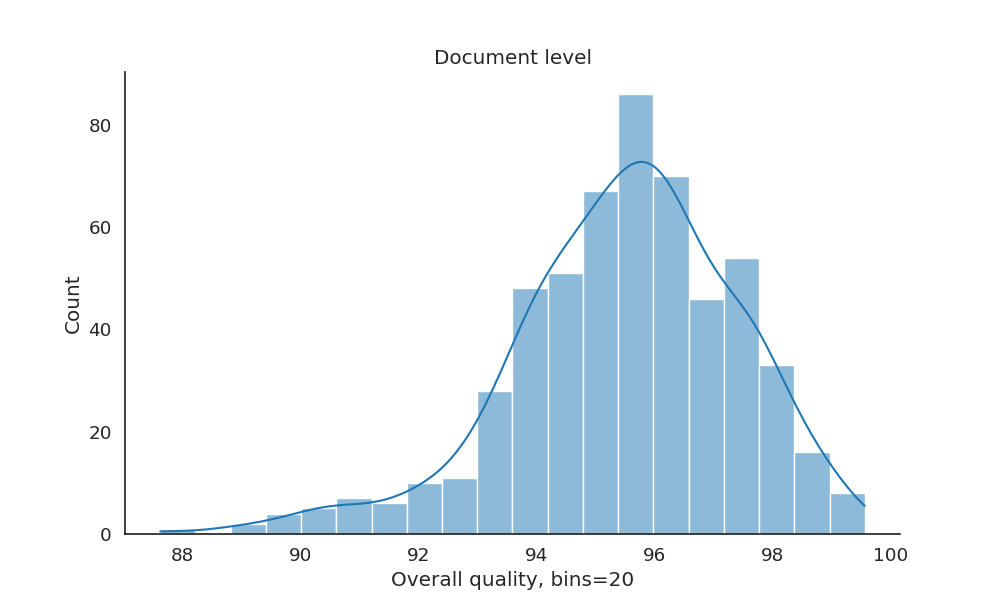
\includegraphics[width=\linewidth]{figures/err/doc-tq-noweights.png}
	\end{minipage}
	\begin{minipage}[c]{0.45\linewidth}
		\centering
		Weighted tq-score
		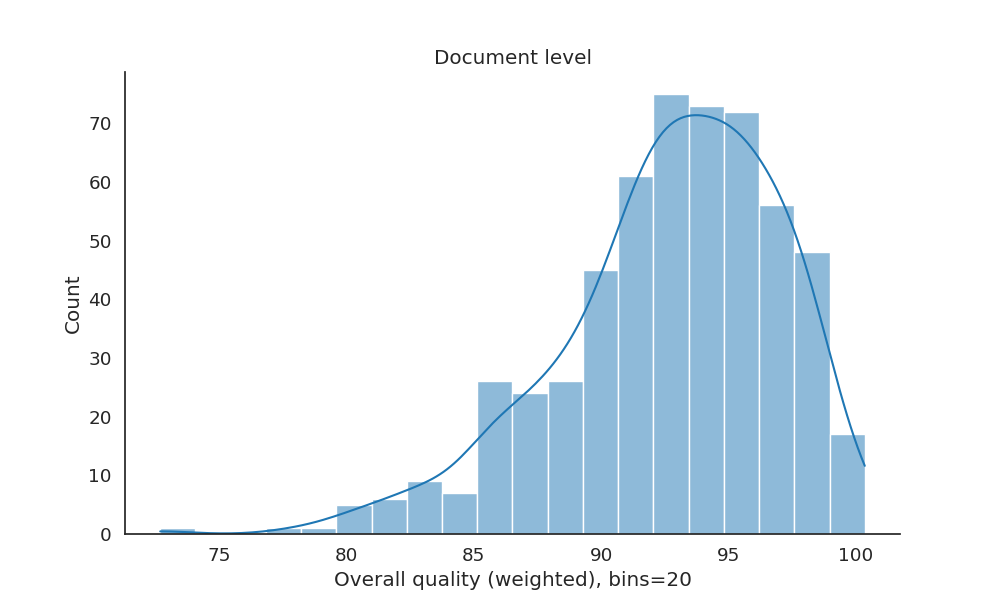
\includegraphics[width=\linewidth]{figures/err/doc-tq-major2critical5weighted.png}
	\end{minipage}	
	\caption{\label{fig:tq}Distribution of overall error-based quality scores for 553 documents}	
\end{figure}

Figure~\ref{fig:docs_fluency} shows that weighting also improves the spread of the data across the measuring scale which should be beneficial for machine learning experiments.

\begin{figure}[H]
	\begin{minipage}[c]{0.45\linewidth}
		\centering
		Unweighted fluency
		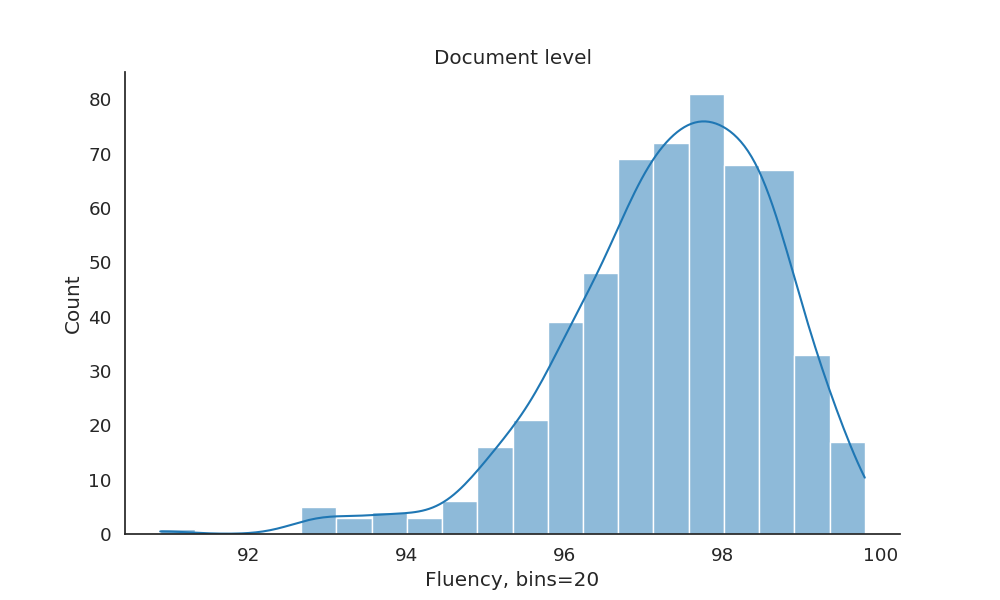
\includegraphics[width=\textwidth]{figures/err/doc-fluency-noweights}
	\end{minipage}
	\begin{minipage}[c]{0.45\linewidth}
		\centering
		Weighted fluency
		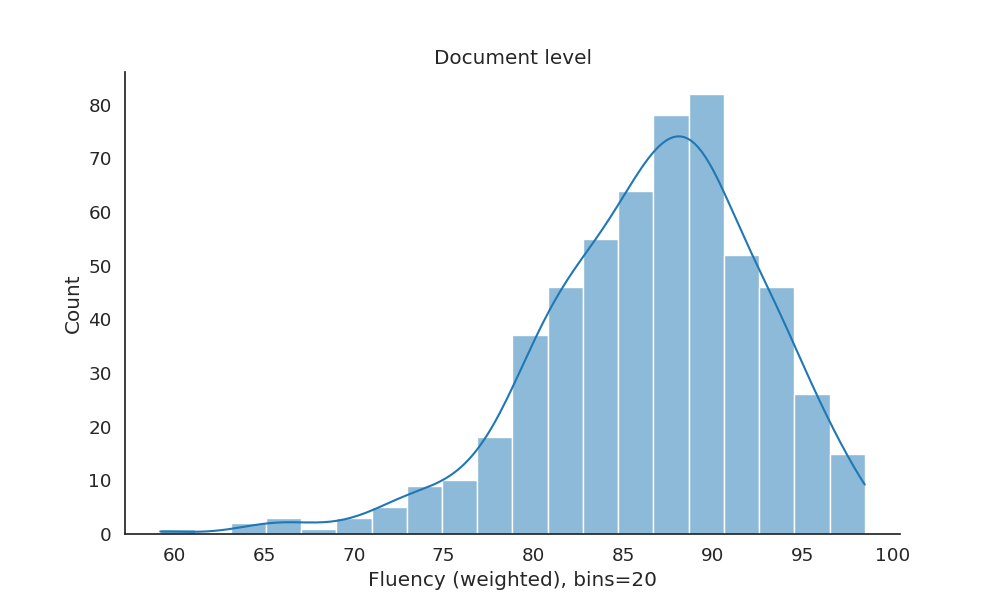
\includegraphics[width=\textwidth]{figures/err/doc-fluency-major2critical5weighted}
	\end{minipage}
	\caption{Document-level fluency scores for quality aspects}
	\label{fig:docs_fluency}
\end{figure}

The same strategy to generating error-based quality scores was applied at sentence level. Out of 12369 sentences in the dataset, 7226 had some sort of annotation (including kudos). While producing sentence-level dataset we skipped 365 sentence pairs that were shorter than three words either on the ST or TT side of the parallel corpus. 

Note that the sentence-level scores reflect issues related to the document texture (cohesion, coherence, logic, etc) if those were located in a given sentence. Care was taken to count errors annotated as discontinuous only once.
\label{pg:skews}
\begin{figure}[H]
	\begin{minipage}[c]{0.5\linewidth}	
		\centering
		Accuracy scores
		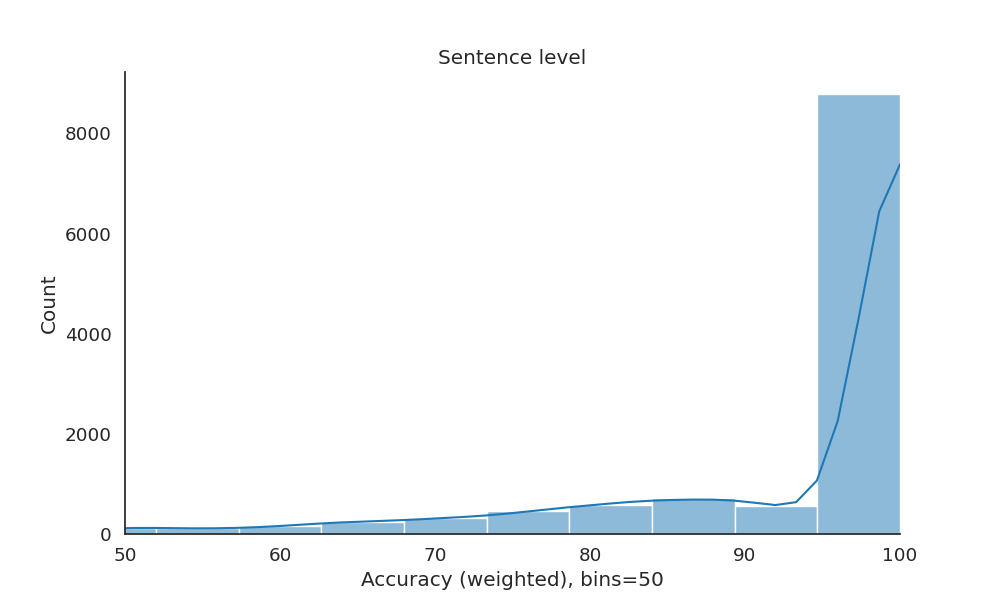
\includegraphics[width=\textwidth]{figures/err/sent-accuracy-major2critical5weighted}	
	\end{minipage}
	\begin{minipage}[c]{0.5\linewidth}
		\centering
		Fluency scores
		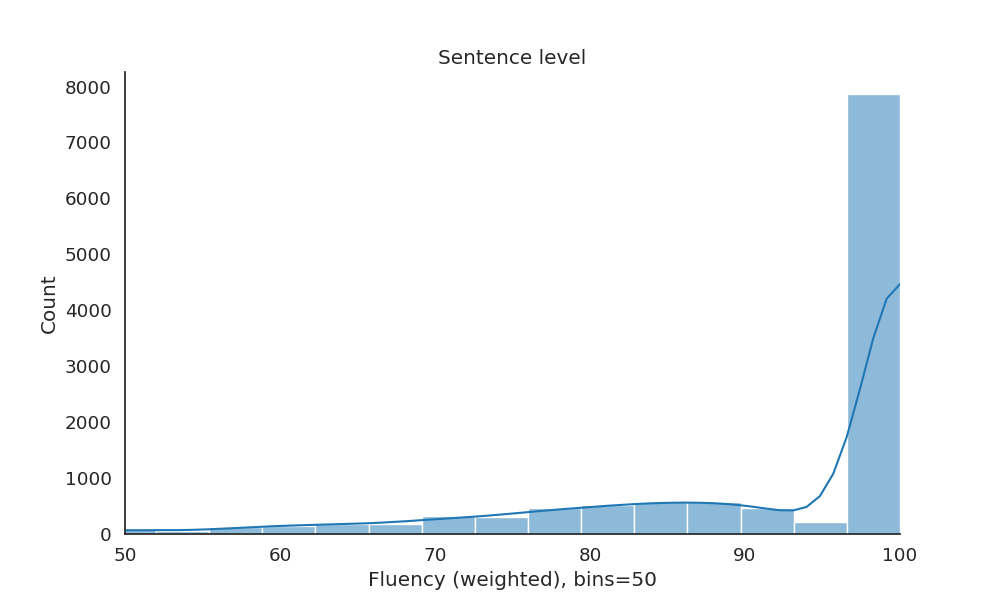
\includegraphics[width=\textwidth]{figures/err/sent-fluency-major2critical5weighted}
	\end{minipage}
	\caption{\label{fig:sents_weighed_aspects}Sentence-level weighted scores for quality aspects: accuracy and fluency}
\end{figure}

\begin{figure}[H]
	\begin{minipage}[c]{0.5\linewidth}	
		\centering
		Unweighted tq
		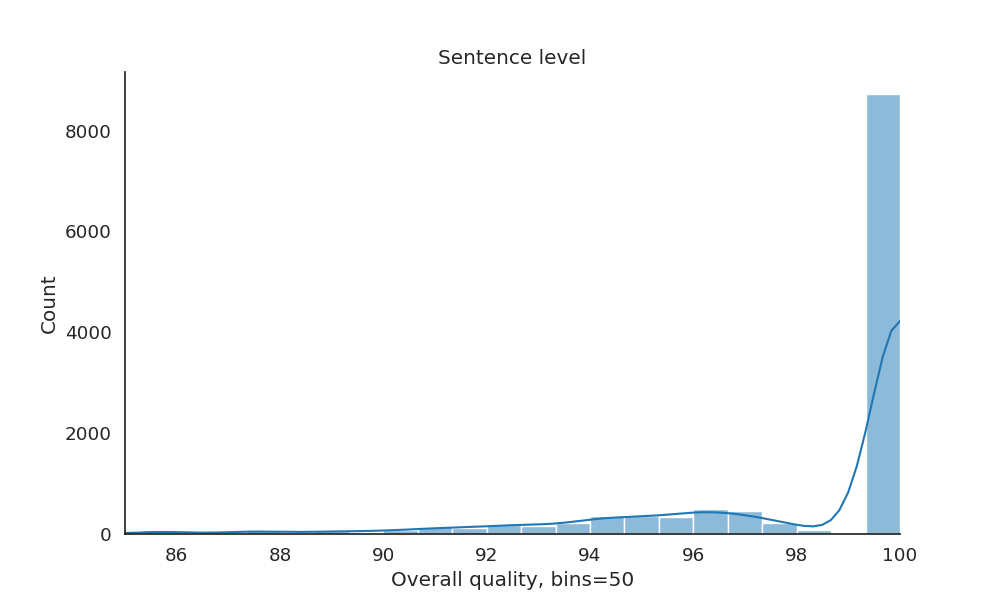
\includegraphics[width=\textwidth]{figures/err/sent-tq-noweights}	
	\end{minipage}
	\begin{minipage}[c]{0.5\linewidth}
		\centering
		Weighted tq
		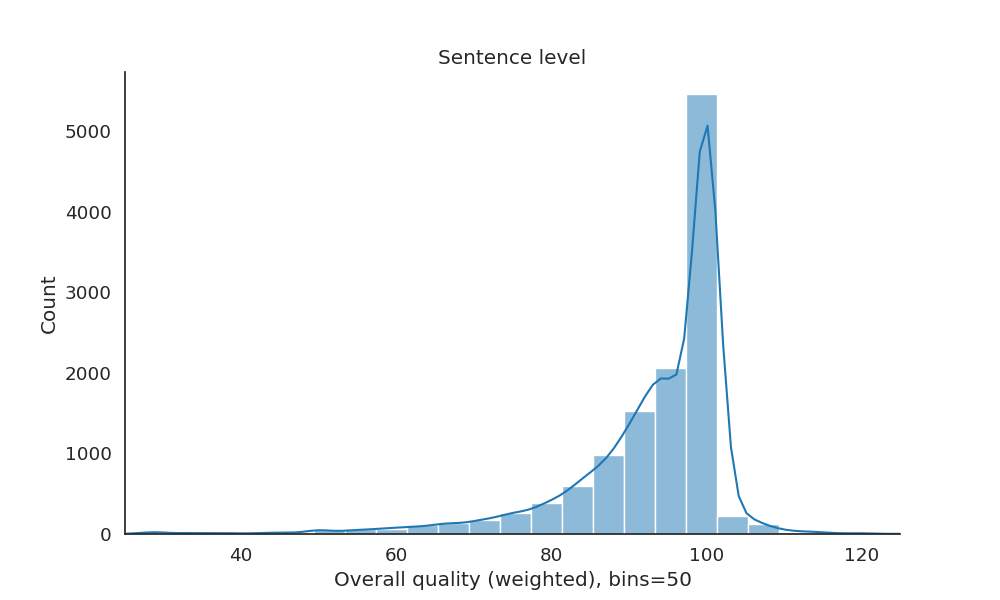
\includegraphics[width=\textwidth]{figures/err/sent-tq-major2critical5weighted}
	\end{minipage}
	\caption{\label{fig:sents_tq}Sentence-level overall quality: unweighted and weighted}
\end{figure}

As can be seen from the histograms in Figures~\ref{fig:sents_weighed_aspects} and~\ref{fig:sents_tq}, sentence-level scores are heavily skewed to the right, which can be a problem for ML algorithms. The distributions of document-level accuracy, fluency and overall quality scores are closer to normality.

\subsection{\label{ssec:da}Direct Assessment}
This section has a description of an annotation project, specifically designed to get quality labels from a controlled experimental setup which follows the requirements and recommendations discussed above.
 
\paragraph{DA experimental setup and results} 
% beware! of is a very skewed output distribution of the DA scores for these particular language pairs.
The Direct Annotation experiment was organised in October 2020 - January 2021. It involved 12 final-year bachelor degree students majoring in Linguistics or Translation Studies (Russian L1, English at least B2). The participants volunteered to do the annotation as part of their internship; the arrangement was approved by the University authorities. The participants were also selected from a larger pool of volunteers following the recommendation their respective course leaders, who characterised them as best of their cohorts (based on academic achievements in their majors). 
The students' work was graded upon the completion of annotation tasks and a written report which contained cross-linguistic analysis of source and target texts with a commentary of translation errors. All participants were using aliases instead of real names throughout the experiment and in all communication of results and progress. 

The experiment was set up on \textit{QuestionPro}\wlvfootnote{\url{www.questionpro.com/}} website, a flexible environment to design online surveys. Following the most recent recommendations for organising quality annotation campaigns by~\citet{Laubli2020}, an annotation task was structured to include the entire document (or coherent extract from large texts) and to present annotators with the source and the target. The annotators were asked to move a slider on a 100-point scale to indicate perceived translation quality.

At the initial stage of the project, there were separate tasks for assessing fluency (in a reference-less monolingual setting) and accuracy (in a bilingual setting). An annotator never received the same document for both settings to avoid familiarity bias. However, the results on control items with `known' quality indicated that annotators struggled with distinguishing the two aspects, and this distinction was abandoned for a syncretic quality judgment. The annotation task was formulated as follows: ``Read the source text. Use the slider to indicate how much you agree that the text in bold is an adequate translation of the original English segment, given the context.'' Figure~\ref{fig:da} has a screenshot of one of the assignments.

\wlvfig[0.4]{da}{Part of a bilingual document and the annotation task}

Before starting on their independent annotation tasks, the participants were explained the purposes of the experiment and had to complete a 30-minutes questionnaire which presented them with a number of translation quality assessment tasks and ensured that they understand the key concepts and terms (e.g. adequate translation, accuracy, fluency, source, target).
Besides, they went through a calibration session to train the participants to use the annotation environment and harmonise the rigour of judgments, while using a slider rather than a Likert scale. 
The calibration results were discussed at a conference and distributed as a written report among the participants.

The independent work was arranged in four stages. At each stage annotators received a batch of 20 annotation tasks, one per document pair. Each complete annotation task (a parallel document of about 21 sentence pairs) was saved separately. The participants were given enough time to complete each batch and were encouraged not to do all 20 tasks in one go.

\label{pg:intersection140}
The documents for annotation were carefully selected from the intersection of the datasets with binary labels and quality scores from error annotation as shown in Figure~\ref{fig:subsets} (page~\pageref{pg:subsets}).

The dataset for annotation comprised 150 multiple translations to 30 English sources, 3,849 unique sentence pairs, including spam items and one repeat document for every participant. 
Spam items were documents with artificially reduced quality to test the integrity and sanity of annotators. Repeat items were exactly the same texts offered to each annotator two months later in a different batch to measure their internal (intra-rater) reliability.

Each source text had 2-3 good and 2-3 bad translations which were never offered in the same batch. In fact, one reason to involve many participants was to avoid presenting an annotator with alternative translations of one source text, at least within one batch, to avoid familiarity bias. To achieve this, we grouped annotators into two teams of six: three translators and three linguists on each team. Each team received their own set of 75 annotation tasks, i.e parallel documents (1,936 and 1,913 sentence pairs for Team 1 and Team 2, respectively). 

To obtain trustworthy annotations, we identified most internally reliable annotators on each team who spotted the spam sentences and returned most consistent results on the repeat items presented to them in different batches. In one of the teams, only two people managed to overcome the established quality control thresholds. Therefore, we had to discard the lower-scoring rater in the other team. Those four raters were treated as interchangeable. This means that the entire dataset had double annotations, half from one team, half from the other team.
% Graham2013: to use the Kappa coefficient to compare agreement levels for the interval-level and continuous scales, we convert continuous scale scores to a target number of interval categories (p.38)
% measure the agreement AFTER standardisation: ``with inter-annotator agreement increasing by up to +0.144 when additional standardization of scores is applied''.
The inter-rater agreement for the document-level annotation achieved weighted Krippendorff's alpha\wlvfootnote{We treated 0-100-point scale as an interval scale and z-transformed values before IRR calculations as recommended in~\cite{Graham2013}} of 0.541 (140 documents, 3,224 sentence-pairs).
% 0.481 for raw scores at document level

For sentence-level, Krippendorff's alpha was 0.463 for z-transformed scores (across 3,224 instances). % 0.440 for raw scores

% 3,557 is the number of sents in 150 files before 10 dropped, there are 3318 sentences in 140 cross-annotated translations, 94 sentences were filtered out as short from sentence level dataset.
Further on, for each team we highlighted individual sentences where both raters returned scores that had more than 30-points difference. Out of 3,318 true instances (sentence-pairs excluding spam and repeat items) in 3,090 cases the raters yielded scores that were less than 30 points apart.
% on average the difference was 3.75, +/-15.73 points BEFORE reworking items. 
% 3318-3090 = 228 difference >= 30 points
The 228 sentences with greater mismatch often were errors in alignment or encoding, and the raters treated them differently. In some translations by-line or date of the publication were omitted in translation, and this led to disagreements. 
%These sentences were fixed and sent for reworking to one of the more reliable raters from the other team. -- Nope, we retain them as is.

\label{pg:final_da}
To get the final scores, we averaged judgments of two raters. Following the practice adopted at \gls{WMT}, the dataset also contains the average of scores z-transformed by rater using Equation~\ref{eq:zscore}. These scores are referred to as \textit{da\_mean} and \textit{da\_zmean}, respectively.

% WMT20 dataset columns: segid	original	translation	scores	mean	z_scores	z_mean	model_scores

\begin{equation}\label{eq:zscore}
\begin{split}
z = \frac{x - \mu}{\sigma} \\
\text{where $\mu$ is mean of the scores by rater,} \\
\text{and $\sigma$ is standard deviation of the respective set of scores}
\end{split}
\end{equation}

Sentence-level datasets with scores from error annotation and from DA experiment were combined to get one dataset with five primary scores (accuracy, fluency, tq, da\_mean, da\_zmean) for intersecting items to enable comparison of the quality scores generated by various methods. 

There were 94 DA-annotated sentences missing from the error-annotated dataset, which was filtered for very short sentences (e.g. \textit{Liquid Gold} -- \cyrillictext{Вода по цене золота} [Water at the price of gold] (RU\_1\_325\_7\_s8); \textit{Right?} -- \cyrillictext{Согласны?} [Agree?] (RU\_1\_268\_4\_s45)).
% Product Placement: On Broadway  Продакт-плейсмент на Бродвее 36.0   100.0
Those sentence pairs were removed from the sentence-level (but not from the document-level!) dataset to ensure consistency.
% Document-level DA scores are calculated from the complete documents.
\begin{table}[H]
	\centering
	\begin{tabular}{l|c|c|cc}
		\toprule
		
		& documents & sentences & \multicolumn{2}{c}{tokens} \\
		\midrule
		&      &        & EN      &  RU \\
		error annotated & 553  & 12,369 & 250,916 & 225,782 \\
		\hspace{1em} inc. with DA & 140  & 3,224 & 62,441 & 57,102 \\
		\bottomrule
	\end{tabular}
	\caption{\label{tab:sent_err_da} Parallel subcorpora with error and DA annotation}
\end{table}

Table~\ref{tab:sent_err_da} brings together the basic quantitative parameters of the dataset with error annotation and DA annotation.
% it was impossible to put sentences with DA and sentences with err-scores into the same df, because a reliable intersection between sent_ids, holding the same (matching) tsent was only 774 tsents out of around 3000. This is because sent_ids were added to err and da texts separately, they went through alignment separately, we deleted items with >= 30 points diff between rater1 and rater 3 (228)

% sent_ids in err and da datasets are mapped to the ame sents, the literal string mismatch is due to the absence of punctuation in "item". We don't use this column anyway.
\label{pg:da_score_hists}
\begin{figure}[H]
	\begin{minipage}[c]{0.5\linewidth}
		\centering
		Document-level
		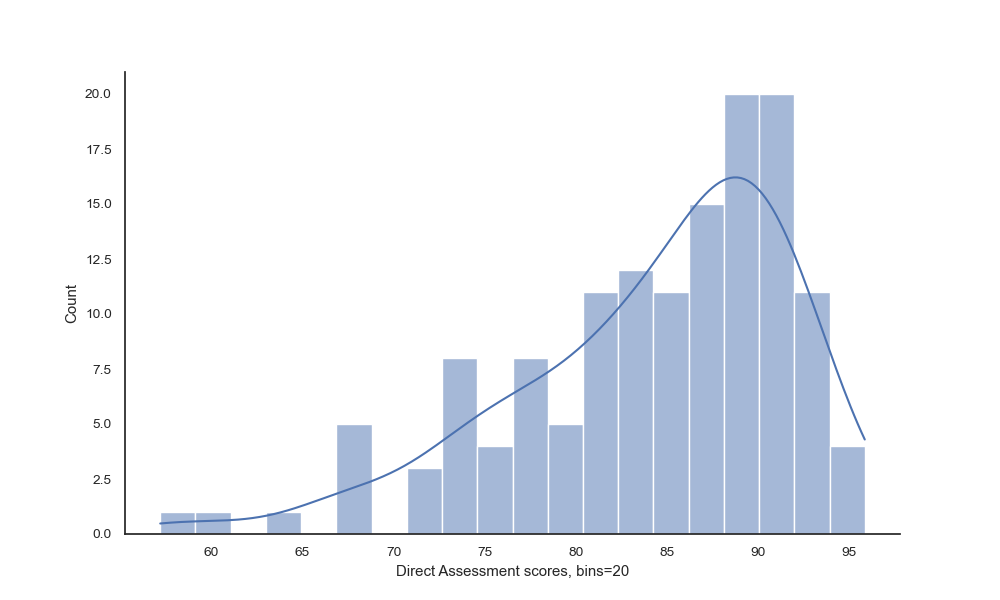
\includegraphics[width=\linewidth]{figures/da/doc-da-score-distribution}
	\end{minipage}	
	\begin{minipage}[c]{0.5\linewidth}
		\centering
		Sentence-level
		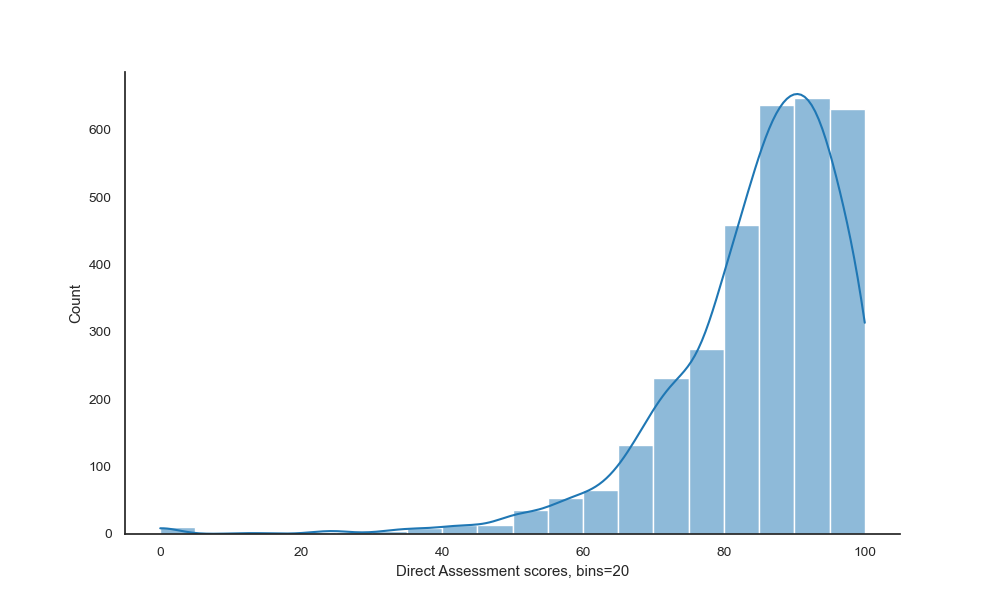
\includegraphics[width=\linewidth]{figures/da/sent-da-score-distribution}
	\end{minipage}
	\caption{\label{fig:da_scores}Distribution of scores from DA experiment for documents and sentences}	
\end{figure}

We provide a visualisation for the distribution of DA scores at document- and sentence-level in Figure~\ref{fig:da_scores}. Similar to scores from error annotation, sentence-level dataset has a more noticeable right skew: there are many more sentences with high-quality scores than with low-quality scores. 


\section{\label{sec:sum4}Summary}

This is a key section in this thesis. It presents the theoretical concept of quality in translation and practical approaches to quality quantification. 
It is focused (i) on automatic quality estimation methods for machine and human translation (Sections~\ref{ssec:mtqe} and~\ref{ssec:htqe} and (ii) on the best practices in producing manual quality benchmarks for NLP experiments (Section~\ref{sec:ass}). The last part of the chapter has a description of annotation procedures used to obtain quality labels and score in this research.
% (Section~\ref{sec:mygold}).

In \gls{TS}, quality is defined with the emphasis on extralinguistic context, including the purpose of translation, intended audience and medium (pragmatic aspect of quality, usually referred to as adequacy). MT research is mostly focused on accuracy and fluency aspects, where accuracy is viewed as (lexico-)semantic similarity between ST and TT, and fluency is approached as readability/grammaticality in the TL. The relative nature of quality was highlighted with regard to three factors, including the purpose of assessment, parameters of communicative situation with translation and comparison with alternative translation candidates. 

Comparing approaches to quality in HT and MT, we have emphasised the limitations of some MT methods due to the predominantly document-level nature of HT, greater variation of language and higher quality expectations attached to HT.

Section~\ref{sec:qe} characterises translation quality estimation as a computational linguistics and NLP task in MT, alternative to reference-based quality evaluation. It can be formulated at various language levels, with sentence level being more practicable for the current MT systems and language representation models. For anyone with the TS background, the idea to assess translation quality on isolated sentences is questionable. 
%Quality estimation tasks predominantly use continuous scores as learning targets. In this case the evaluation studies rely on correlation coefficients and error rate metrics to compare the performance of various methods. When quality of translations is captured by discrete labels, systems' evaluation is based on typical ML classification metrics: accuracy, precision, recall and F-score. 

This chapter offers an overview of the current best-performing approaches in MTQE and summarises the two projects that attempted to extend MT estimation methods to HT. We demonstrate that current state-of-the-art in MTQE relies on pre-trained contextualised embeddings fine-tuned on quality labelled data, and researchers' attempts are focused on explainability. Document-level MTQE task waits for further advances in technology to be successfully tackled and builds appropriate datasets meanwhile. 
We include a critical description of a popular MTQE feature set from \textit{QuEst++} used as a baseline in this research.  

Document-level HTQE based on a careful selection from a elaborate set of 360 types of hand-engineered surface features achieved Pearson's $r=0.72$ outperforming \textit{QuEst++} on the dataset proposed in Yuan's \citeyear{Yuan2018} research. In their experiments feature-learning approach was inferior to explicit features at sentence level. However, a critical analysis of their learning setup (in particular, very repetitive translations for a very few STs) warrants doubts about robustness of this approach.
The other research casts HTQE as an unsupervised sentence-level task based on learning similarity between ST and TT.
 
The last two sections of this chapter discuss the second component of any quality estimation task -- quality labels. 
We present a fairly detailed analysis comparison of reliability and application of the major competing assessment methods in HT (rubrics and error annotation) and in MT (error annotation, direct assessment, post-editing). It has been repeatedly emphasised that when it comes to collecting human judgment about translations, it is best to resort to professional expertise, provide a rigorously formulated definition of quality for each text type/communicative situation and have a calibration strategy in place. The latest recommendations also require translations to be assessed in the true document order.
In MT there is more awareness that these methods capture various dimensions of quality, and there is more pessimism about getting humans to agree about quality. It is obvious that in MT there is a pressure to adjust quality benchmarking methods to the changes in MT quality delivered by the introduction of NMT. 
%In our opinion, lower inter-rater reliability results in MT can be explained by non-professional annotators, who look at an isolated sentences. 
We tend to agree that the distinction between aspects of quality (accuracy and fluency) is even more difficult to capture in an annotation experiment. 

While describing the best practices in producing quality benchmarks in MT we focus technical details, such as the choice of top-level error categories, use of severities, ways to convert error statistics to actual quality scores and annotation environments. 
A separate subsection discusses organisation of reliability studies for various annotation setup. We note that measuring IRR for error annotation or post-editing is particularly difficult because ideally it involves taking into account the agreement about the location of the annotated spans and their categorisation. Further caveats heeded in our own experiments include the recommendation to use Krippendorff' coefficient in IRR studies and to apply metrics to z-transformed (standardised) DA scores instead of absolute values. 
 
It was also repeatedly shown that the outcomes of supervised ML experiments are contingent on the distribution of scores in the dataset. 

Finally, we provided detailed descriptions of three annotation procedures used to obtain or verify various quality labels/scores in our datasets. The results were reported in terms of IRR and scores distribution at document and sentence levels. We demonstrated that in our various experiments the agreement between university translation teachers (nominal-scale assessment and error annotation) and final-year under-graduate students (DA experiment) as raters ranges from 0.467 to 0.734 in various settings, with the lowest result seen for sentence-level DA by students.
